\documentclass[pdflatex,sn-mathphys-ay]{sn-jnl}
\usepackage{iftex}
\ifPDFTeX
\usepackage[T1]{fontenc}
\usepackage[utf8]{inputenc}
\usepackage{newtxtext}
\else
\usepackage{fontspec}
\setmainfont{Times New Roman}
\fi
\usepackage{amsmath,amssymb}
\usepackage{graphicx}
\usepackage{booktabs}
\usepackage{array}
\usepackage{float}
\usepackage{xurl}
\usepackage[final]{microtype}
\usepackage{tabularx}

\makeatletter
\providecommand{\headerps@out}[1]{}
\providecommand{\theHfigure}{}
\providecommand{\theHtable}{}
\renewcommand{\email}[1]{\global\advance\emailcnt by 1\relax%
\if@corauemail%
	\g@addto@macro\corrauthemail{%
	\setcounter{footnote}{0}%
	{\normalfont\ttfamily\small\textcolor{black}{\nolinkurl{#1}}};\space%
	}%
\else%
	\g@addto@macro\authemail{%
	\setcounter{footnote}{0}%
	{\normalfont\ttfamily\small\textcolor{black}{\nolinkurl{#1}}};\space%
	}%
\fi}
\renewcommand{\theHfigure}{\arabic{figure}.\arabic{page}}
\renewcommand{\theHtable}{\arabic{table}.\arabic{page}}
\AtBeginDocument{\hypersetup{hypertexnames=false}}
\makeatother

\emergencystretch=2em
\raggedbottom
\vbadness=10000
\hfuzz=2pt

\begin{document}

\title[Women's Entrepreneurship and Agricultural Lending]{The Impact of Agricultural Lending on Women's Entrepreneurship in Kazakhstan's Agricultural Sector: The Role of Regional Factors and Access to Land}

\author[1]{\fnm{T.} \sur{Arzayeva}}\email{talanttyarzayeva@gmail.com}

\author*[1]{\fnm{B.} \sur{Aimurzina}}\email{aimurzina2016@gmail.com}

\author[1]{\fnm{Zh.} \sur{Bulakbay}}\email{bulakbay_zhannat@mail.ru}

\author[1]{\fnm{G.} \sur{Mataibaeva}}\email{mataibaevagauhar@mail.ru}

\author[1]{\fnm{R.} \sur{Sadvakassov}}\email{sadvakasov.rm@gmail.com}

\affil*[1]{\orgname{L.N. Gumilyov Eurasian National University}, \orgaddress{\city{Astana}, \country{Kazakhstan}}}

\abstract{Women's entrepreneurship in agriculture is recognized as an important factor in inclusive growth; however, empirical data on the transition economies of Central Asia remain underresearched. This study analyzes the causal influence of institutional agricultural lending on the development of women-owned farms in 20 regions of Kazakhstan over the period 2015--2024 (175 observations). We employ a three-module analytical approach: (1) two-way fixed-effects (TWFE) panel regressions to identify causal relationships; (2) k-means clustering to account for regional heterogeneity; and (3) the random forest method to assess the predictive power of variables. Access to credit does not have a statistically significant causal effect on the number of female-headed farms in the region after controlling for fixed effects, despite a positive correlation in the combined model (pooled OLS). The clustering results revealed that the regions fell into two distinct groups. The first is characterized by a high level of female farming, but growth in this group is low. In the second group, the initial indicators are significantly lower, but the growth rate is three times greater. However, in neither group do we find evidence that lending specifically drives this dynamic. In our view, another factor, access to land, proves to be significant. On average, across the sample, women own only 2.01\% of agricultural land (median: 1.19\%), which is an institutional factor limiting female entrepreneurship. The findings indicate that simply increasing the volume of lending is not enough to solve the problem. The key points highlighted by these data are the need to account for regional differences and institutional barriers. These barriers, rather than a lack of lending, hinder the development of women's entrepreneurship. This necessitates differentiated, region-specific measures that combine financial instruments with reforms in land rights and regional infrastructure.}

\keywords{agricultural lending, women's entrepreneurship, financial inclusion, regional heterogeneity, Kazakhstan, inclusive development, access to land, land access}

\pacs[JEL Classification]{Q14, J16, O13, Q12, O15}

\maketitle

\section{Introduction}\label{sec:introduction}

Women's entrepreneurship in agriculture is increasingly recognized as a key driver of inclusive economic growth, rural development, and ensuring food security in both developing and transition economies \citep{ref78}. Amid the global transformation of agricultural systems, ensuring women's equal access to resources (land, finance, and technology) is becoming not only a matter of social justice but also a prerequisite for increasing the sector's overall productivity \citep{ref62,ref26}.

Kazakhstan, a country that has maintained a significant state role in agricultural financing, implements large-scale institutional lending programs through KazAgroFinance JSC, the Agrarian Credit Corporation JSC, and the Fund for Financial Support of Agriculture JSC. The proportion of women who head farms, according to the Bureau of National Statistics, remains low despite loans (on average, only 2.01\% of agricultural land is registered to women (with a median of 1.19\%)).

The question of how access to financing affects farmers' performance has been widely studied in the literature \citep{ref94,ref99}. However, when examining the situation, most empirical studies have methodological limitations:

\begin{itemize}
\item the data are based on cross-sectional data. This makes it impossible to distinguish correlation from causation: we observe a pattern but do not know what influences it;
\item the geographical scope of the studies is concentrated on countries in Africa and South Asia, whereas post-Soviet countries, with their unique institutional structure, have been virtually unexplored;
\item There is a lack of research examining the relationship between lending and access to land. This combination may be key for women farmers, as our preliminary data show.
\end{itemize}

This study addresses these gaps by analyzing panel data from 20 regions of Kazakhstan over a 10-year period (2015--2024, 175 farms). The contributions of this work are as follows. First, we identify the reasons why institutional agricultural lending influences the development of women-owned farms in the Central Asian context. Second, we employ a three-module analytical approach, namely, fixed-effects panel econometrics, cluster analysis, and machine learning methods, to disentangle interregional correlation and the causes of intraregional and regional heterogeneity. Third, we empirically test the hypothesis that access to land acts as a binding institutional constraint that reduces the potential impact of financial support.

On the basis of theoretical analysis and identified gaps in the literature, this study tests the following hypotheses:

H1: Access to institutional agricultural lending has no statistically significant effect on the number of women-owned farms within regions.

H2: The relationship between lending and the outcomes of women's entrepreneurship is heterogeneous and varies depending on the level of infrastructure development and the institutional capacity of regions.

H3: Access to land (land\_share) positively moderates the effect of lending, but its institutional limitations (on average, 2.01\% of land) reduce the overall effectiveness of financial support.

The empirical strategy is based on an unbalanced panel combining data from the National Statistics Bureau of the Republic of Kazakhstan, state agricultural financial institutions, and the Land Resources Management Committee. We estimate two-way fixed-effects (TWFE) models with clustering of standard errors at the regional level, apply k-means clustering to identify stable regional regimes, and use random forest with group cross-validation to assess the predictive power of the variables.

The remainder of the article is structured as follows: Section 2 contains a literature review and the conceptual framework of the study. Section 3 describes the data, variables, and three-module analytical framework. Section 4 presents the results of the empirical analysis. Section 5 discusses the findings in the context of existing research. Section 6 presents conclusions for Kazakhstan's agricultural policy. Section 7 concludes the article.

\section{Literature review: a critical synthesis}

\subsection{Theoretical foundations of inclusive development}

Ensuring equal access to resources for all participants in agricultural
production is defined in international studies as a strategy for
inclusive development \citep{ref29,ref44,ref77}. However, this general understanding masks
significant disagreements. The question of exactly how inclusivity
should be implemented is a subject of disagreement among authors.

\citet{ref81} emphasized inclusivity in the value chain.
\citet{ref24} noted that innovations in gender development are key
methods for sustainable agricultural development. \citet{ref27}
highlights the crucial role of women's empowerment and its impact on
household agricultural productivity.

One such point of contention concerns the role of partnerships between
large agribusinesses and small-scale producers. Some researchers view
these partnerships as the primary driver of inclusive growth
\citep{ref34,ref90}. In contrast, others show that, in practice, large farms dictate the terms, putting
small producers at a disadvantage \citep{ref90}.

An even more heated debate has emerged around technological innovations.
\citet{ref105}; \citet{ref72}; \citep{ref43,ref37,ref104} argue that digitalization and
artificial intelligence can increase access to resources. Without
accompanying institutional reforms, technological interventions are
likely to exacerbate inequality, according to \citet{ref28},
with the primary benefits going to the most resource-endowed producers.
Our study takes a middle ground: we do not dismiss the potential of
financial instruments, but we empirically test the conditions under
which they are effective.

Issues related to public policy aimed at strengthening the digital
financial services infrastructure in rural areas to ensure high-quality
and sustainable growth in agricultural production are addressed in the
study by \citet{ref38}. Modern approaches to agriculture
require the integration of multidimensional models that consider not only
production indicators but also parameters of
sustainability, inclusivity, and environmental integrity.

Many aspects of inclusive development are systematized in the work of
\citet{ref55}, which identifies five key areas for the
inclusive transformation of rural areas: (1) renewing long-term
investment in research and development, taking into account the
principles of equality and gender parity; (2) taking into account the
interests of marginalized groups; (3) ensuring equal access to
technologies; (4) levelling the conditions of competition by limiting the
dominance of large corporations and supporting small and medium--sized
agribusinesses; (5) prioritizing employment development in the context
of automation and the expansion of value chains.

\citet{ref47}, \citet{ref64}, and \citet{ref96} noted that structural changes in rural
regions depend on the inclusiveness of these processes. Climate impacts
and low productivity are obstacles to the sustainable transformation of
rural areas. Two mechanisms that promote inclusive development ---
investment in human capital (healthy nutrition and education) and the
equitable distribution of resources and reduction of risks for
vulnerable populations --- can lead to social well-being but require
coordinated policy measures, according to \citet{ref21}.

Its main areas of activity include coordination of the agricultural and
nonagricultural sectors, development of digital infrastructure in rural
areas, and, equally importantly, the integration of principles of
inclusivity into the modernization processes themselves.

An examination of the theoretical sources of inclusive agricultural
development has allowed us to identify several key points.

There is no consensus on exactly how inclusivity should be implemented.
Some authors emphasize value chains \citep{ref81}, whereas
others focus on innovation and the advancement of gender equality
(Dabkienė, 2025) and on measuring women's empowerment and its impact on
productivity (Doss, 2025). Using a three-module analytical approach, we
emphasize the need for a comprehensive, multidimensional assessment of
inclusivity.

A contradiction in the assessment of the role of large agro-industrial
enterprises. Partnership with large
companies is viewed as a driving force for inclusive growth
\citep{ref34}, whereas others show that large farms dictate terms,
exacerbating inequality among smallholder farmers \citep{ref90}.

Discussion surrounding technological and digital innovations as a means
to expand access to resources \citep{ref105,ref43,ref37} and
institutional reforms \citep{ref28}.

\citet{ref55} identifies five key areas for the inclusive
transformation of rural areas, including addressing the interests of
marginalized groups and ensuring equal access to technology.

A review of the theoretical framework revealed that inclusive
agricultural development depends on institutional conditions,
technological infrastructure, and social mechanisms. The identified
contradictions justify the need for our study, which focuses on two key
factors: access to credit (financial mechanism) and access to land
(institutional barrier).

\subsection{Financial inclusion: correlation and causality}

In existing studies, expanded access to financial resources is
predominantly viewed as an important factor in entrepreneurial growth
\citep{ref103}.

A positive correlation between the volume of lending and agricultural
growth has been demonstrated in the following studies
\citep{ref94,ref99,ref70,ref49,ref95,ref97,ref61}.

We identify three methodological limitations:

\begin{itemize}
\item Most cross-sectional studies are based on cross-sectional
surveys, making it impossible to identify the causes of correlations;
\item the authors of these studies and their geographical focus are
concentrated primarily in African countries and South Asia
\citep{ref90,ref58,ref42,ref71,ref44,ref97,ref84}. Post-Soviet countries, including Kazakhstan, with their
unique institutional legacy, remain outside the scope of this analysis.
However, their experience may differ significantly;
\item Institutional constraints are overlooked. Research on financing
rarely addresses access to land. However, for the agricultural sector,
land is not only a productive resource but also a key collateral asset
\citep{ref20,ref06}. Without taking this factor into
account, the research is unlikely to be comprehensive.
\end{itemize}

However, there is one exception. \citet{ref18} proposed
flexible risk management tools tailored to households' resource
capacities. Unfortunately, the question of whether this approach is
applicable to women's entrepreneurship has not been addressed.

Digital financial instruments deserve special attention. Researchers see
potential in them: digital integration can reduce transaction costs and
make financing more accessible. However, the extent to which this
potential is realized for women farmers in post-Soviet countries has not
been fully explored.

\citet{ref63} and \citet{ref76} identified several factors
hindering the development of the agricultural sector. These include
outdated technologies and farming methods, an inefficient financing
system, unstable farm incomes, low liquidity of collateral, and a lack
of technological and financial support. Each of these factors deserves
separate attention.

The issue of where agriculture remains a priority is pressing for
Kazakhstan. Government policy is focused not only on developing the
financial sector; this year was declared the year of digitalization in
Kazakhstan. This is being done to address issues such as the
reallocation of resources in agriculture, infrastructure development,
and expanding access to lending, primarily for small farms, through the
use of digital inclusive finance as an alternative to traditional forms
of support. These aspects are addressed in the works of many scholars
\citep{ref56,ref80}.

The key role of digital finance in promoting the sustainable development
of rural regions was explored by \citet{ref87}.
The authors demonstrate that investment in digital infrastructure is
necessary to ensure the sustainable modernization of the agricultural
sector.

In developing countries, modernization is often constrained by a
combination of resource and institutional limitations. In response,
comprehensive programs have emerged. Governmental and nongovernmental
organizations combine the provision of loans with training for farmers
\citep{ref74,ref13,ref73}.

These studies have a methodological shortcoming: they fail to
distinguish between interregional correlation and intraregional
causality. In this study, we propose a different methodological
approach, using panel data for 20 regions of Kazakhstan over a 10-year
period and a fixed-effects model (TWFE).

\subsection{Gender barriers: an institutional approach}

In our view, two competing approaches can be identified in the
literature on gender development in agriculture.

The financial approach \citep{ref60,ref88} emphasizes expanding access to microfinance and banking
services as a key mechanism for women's empowerment. This finding demonstrates a
positive correlation between access to finance and entrepreneurial
outcomes.

Financial instruments are ineffective without addressing issues of land
rights, market access, and participation in decision-making. This is a
key feature of the institutional approach outlined in previous works
\citep{ref78,ref26,ref02,ref32,ref36,ref66}. Credit alone
cannot stimulate sustainable growth.

Barriers to access to land and credit were identified by
\citep{ref26,ref20,ref06}, who compared the
relative importance of financial and institutional constraints and
justified the need for land rights. However, the institutional
environment in which they are studied differs from that existing in the
Kazakhstan's economy.

In summary, ensuring gender equality and social integration in
agriculture can be described as follows:

From production processes to social relations and institutional
mechanisms is the subject of academic debate \citep{ref78,ref93,ref04}. Successful inclusion
requires taking the gender dimension into account throughout the entire
process, from planning to monitoring.

We found a study of a systemic approach closely linked to inclusive
agricultural development and financial support instruments for various
agricultural groups, including women, in the article by \citet{ref48}. Other authors, such as \citet{ref11},
characterized women's entrepreneurship as ``family business''. The
promotion of women's active participation in leadership roles, leading
to a reduction in social inequality in rural areas through the use of
special measures, is reflected in the work of \citet{ref82}.

We identify two key points in these studies. The advancement of women,
who possess a diverse range of skills and knowledge, contributes to
economic stability, innovation, and the promotion of sustainable
development in rural areas \citep{ref82}. \citet{ref75}, and \citet{ref02}, supplemented the first point
with the need for access to land, productive resources, finance,
markets, and the creation of added value through cooperatives.

Gender equality not only drives innovative and social processes in
agriculture but is also linked to the green economy and effective
governance policies. This is highlighted by the following authors:
\citet{ref57}; \citet{ref31}; \citet{ref05}; \citet{ref106}.

Farms managed by women are more likely to adopt agroecological practices
and create sustainable food systems, thereby receiving more subsidies,
increasing crop yields, and demonstrating a high level of autonomy,
according to \citet{ref67}, and \citet{ref50},
a view with which we cannot help but agree.

\citet{ref92} added another important dimension.
Sustainable development in agribusiness is impossible without equal
access to clean natural resources, socioeconomic benefits, and social
protection. In their view, this is a crucial aspect of inclusive rural
development.

All of these findings lead to one conclusion: gender-oriented policies and
support programs are not merely supplementary but necessary conditions
for inclusive and sustainable agricultural development. \citet{ref20} empirically confirms this conclusion. The study shows that
access to land rights has a positive effect on productivity and income
but is often overlooked in policy-making.

Secured land rights empower women by enabling them to invest in
agriculture and adopt improved farming practices. For Kazakhstan, where
systemic barriers to female farmers persist, these findings have direct
practical implications.

Notably, women's access to microfinance
\citep{ref60} leads to their empowerment, improved
living conditions, and better decision-making; therefore, it is
necessary to conduct a more in-depth study of socioeconomic issues and
ways to address them.

According to \citet{ref91}, other factors
motivating rural women to start their own businesses include a desire
for independence, fair pay commensurate with the amount of work, and
entrepreneurial skills.

In addition, women-led microenterprises, which form the backbone of
rural communities and contribute to economic growth and sustainable
development, often face significant challenges, particularly in securing
financial support and establishing stable social networks \citep{ref14}.

According to \citet{ref68} and \citet{ref46},
women's empowerment is linked to increased agricultural productivity and
poverty reduction. Building on this idea, \citet{ref94},
\citet{ref88}, and \citet{ref16} noted that
access to lending and household economic status, as well as support for
women entrepreneurs, have a positive and significant impact on
entrepreneurial success.

\citet{ref35}, \citet{ref23}, and \citet{ref62} identify two key barriers for women entrepreneurs in
agriculture: limited access to finance and inadequate infrastructure.
Without addressing these, the authors conclude, business growth and
sustainability are unlikely.

\citet{ref99} demonstrated how high the potential of
agricultural entrepreneurship is. This includes income, food security,
sustainable development, overcoming gender stereotypes, and job
creation. The list is impressive.

However, realizing this potential, as noted by \citet{ref25},
and \citet{ref85}, is hindered by the same obstacles:
limited access to financing, education, and training. Until these
barriers are removed, the positive effects described by \citet{ref99}, will remain largely theoretical.

\citet{ref89}, and \citet{ref19},
emphasize that women's entrepreneurship is not merely a social issue. It
is a key factor in economic development and the empowerment of women,
particularly in rural areas.

In summary, the issue of gender inequality stems
from fundamental systemic constraints, which can be categorized as
follows: access to land \citep{ref39,ref06,ref102,ref52,ref12} and women's participation in governance and decision-making
\citep{ref79,ref40,ref08,ref09,ref69}. The findings of this literature review
confirm the validity of an institutional approach to analyzing women's
entrepreneurship in the agricultural sector.

\subsection{Regional heterogeneity: a gap in the literature}

Most studies on financial inclusion assume that the impact of lending is
universal. It either ``works'' or ``does not work,'' regardless of the
region, infrastructure, or institutional context.

However, \citet{ref21} and \citet{ref17}
noted important nuances. The effectiveness of financial
instruments largely depends on additional investments in infrastructure,
education, and market institutions.

The problem is that this aspect remains understudied. Two reasons can be
identified. The first is methodological. Studies using cluster analysis
to identify regional development patterns are extremely limited.

The second is empirical. Studies combining econometrics and machine
learning methods applied to the agricultural economy are virtually
nonexistent.

Our study aims to fill this gap. We integrate three analytical modules
-- TWFE, k-means, and random forest. This allows us not only to identify
regional heterogeneity in Kazakhstan but also to assess the robustness
of the results obtained.

Aspects of the issues related to the impact of credit on women farmers
in the Kazakhstan economy, which has its own specific characteristics,
remain understudied, which reinforces the relevance of our research. We
examined methodological approaches to assessing the impact of various
types of credit on the economic situation of women in agriculture based
on the works of \citet{ref10}, \citet{ref03}, \citet{ref30}, \citet{ref41}, and \citet{ref59}.

There are also few studies by domestic researchers on this topic. The
impact of women's entrepreneurship on economic growth was examined in
the works of \citet{ref07}, \citet{ref15}, and \citet{ref51}.

We integrate the technological and institutional approaches examined in
the literature review to assess how lending interacts with an
institutional factor such as women farmers' access to land. Our study
differs from previous studies in that we attempt to empirically test
whether credit support from financial institutions in Kazakhstan can
compensate for limited access to land. Or does access to land remain a
binding constraint that reduces the impact of lending?

\section{Research methodology}

1. The systematic logic of the study's design ensures a phased approach to addressing the following tasks: first, the presence of a causal relationship is verified (panel econometric analysis \citep{ref22,ref53,ref101}), then the structural context of the phenomenon is revealed (cluster analysis), and in the final stage, the predictive significance of the results is confirmed (machine learning methods).

\begin{figure}[H]
\centering
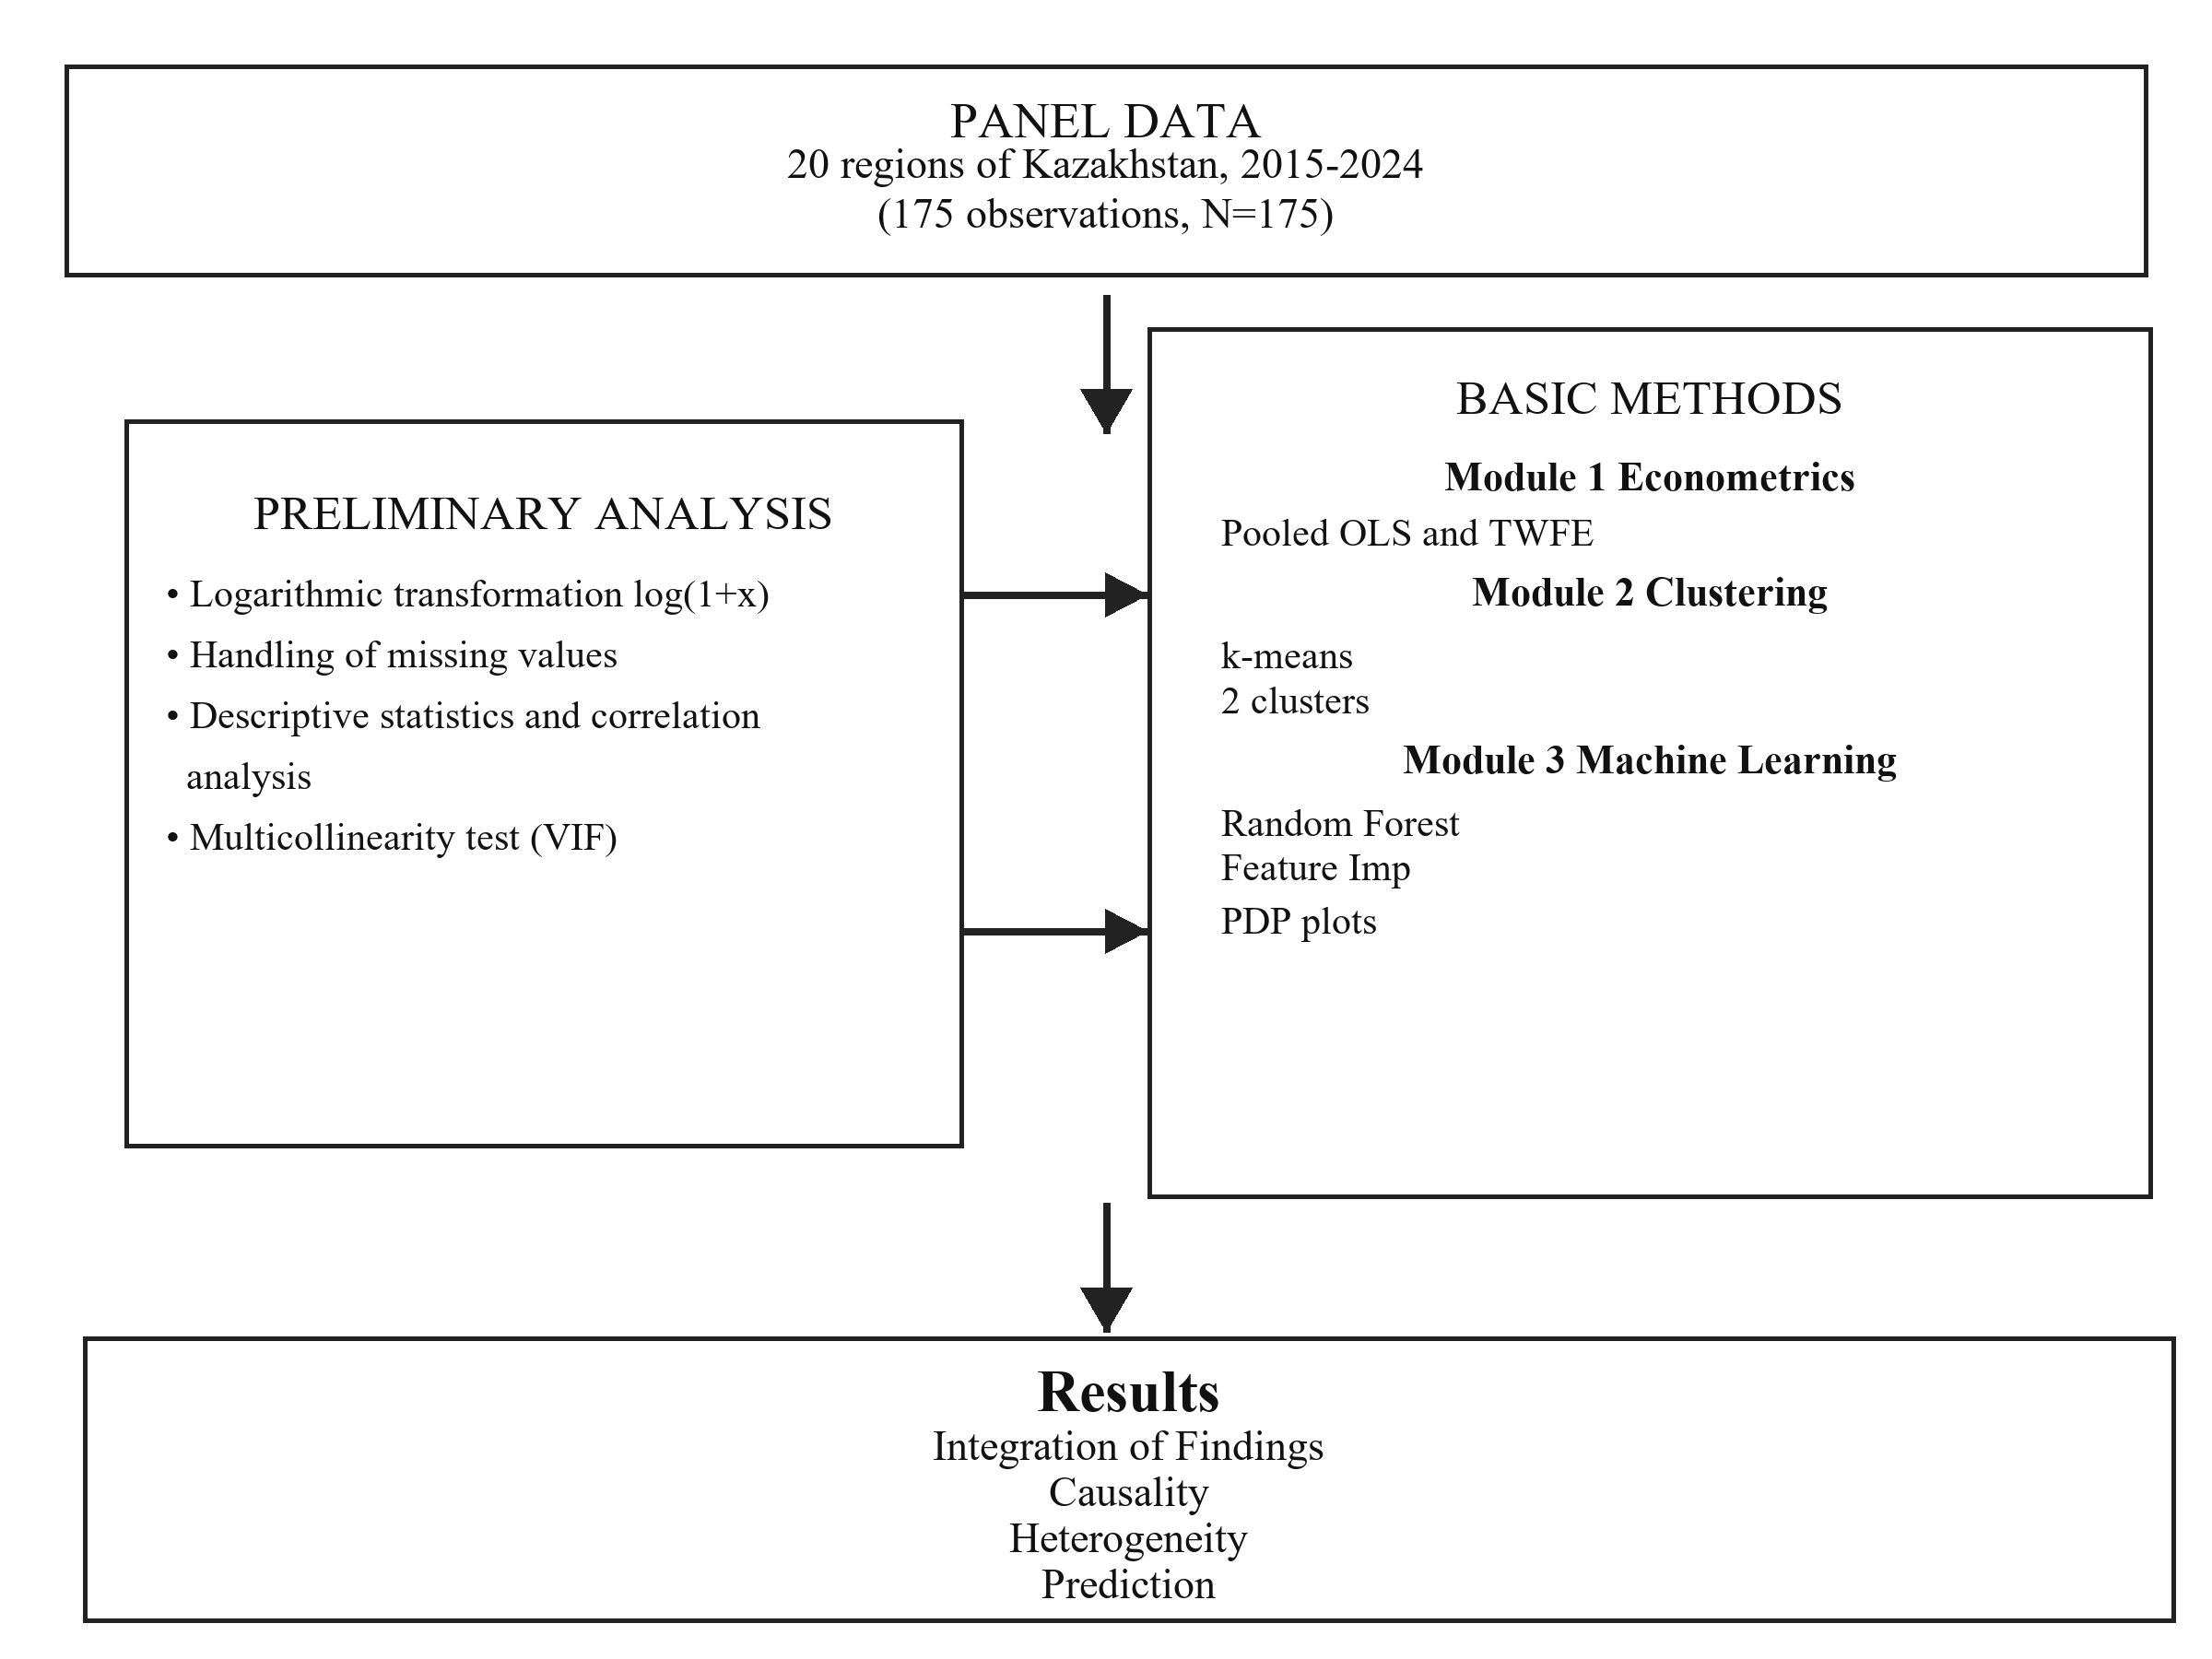
\includegraphics[width=\linewidth,keepaspectratio]{figures/figure01.png}
\caption{Research design: three-module analytical framework}
\label{fig:research-design}
\end{figure}

The analysis is based on unbalanced panel data for 20 regions of
Kazakhstan covering the period 2015--2024, totaling 175 observations.
The spatial unit is the region, and the temporal unit is the year.

Data sources: National Statistics Bureau of the Agency for Strategic
Planning and Reforms of the Republic of Kazakhstan https://stat.gov.kz/:

\begin{itemize}
\item Data on women-owned farms and agricultural lending: KazAgroFinance
JSC, Agrarian Credit Corporation JSC, and the Agricultural Financial
Support Fund JSC for 2015--2024: (Women and men of Kazakhstan.
Statistical compendium)
\item Land use data from the Land Resources Management Committee of the
Ministry of Agriculture of the Republic of Kazakhstan: ``Proportion of
women provided by agricultural land, broken down by form of ownership''
(2015--2024).
\end{itemize}

The dataset includes variables characterizing the number of women-owned
farms, the volume and sources of agricultural lending, and women's
access to land resources. A detailed description of the
variables is presented in Table 1.

\subsection{Description of variables and transformation}

A logarithmic transformation was applied to bring the data to the
econometric model. The transformation log(1 + x) was used for the
variables women\_farms and the lending indicators. This approach
normalizes the distribution and allows the regression coefficients to be
interpreted as elasticities (the percentage change in the dependent
variable for a 1\% change in the independent variable). The choice of
the log(1+x) transformation is due to the presence of zero values in
some components of lending.

The dependent variable is defined as:

log\_women\_farms -- the logarithm of the number of active farmer farms
headed by women.

Key independent variables:

log\_credit\_total -- the logarithm of the total volume of institutional
agricultural loans issued to women (the sum of the three components).

log\_credit\_kaf -- the logarithm of loans issued by KazAgroFinance JSC.

log\_credit\_acc -- the logarithm of loans issued by Agrarian Credit
Corporation JSC.

log\_credit\_fund -- the logarithm of loans issued by Agricultural
Financial Support Fund JSC.

lag1\_log\_credit\_total -- first-order lag of the total lending volume
variable (previous year's value) to assess the lagged effect.

Control variables:

land\_share -- the share of agricultural land allocated to women (as a
percentage of the total agricultural land area in the region), which is
important for distinguishing between the effects of credit and land
ownership.

Identifiers:

region\_id - numerical region identifier (1--20).

year - observation year (2015--2024). (The data are presented in Table 1.)

Handling of missing values:

An analysis of data completeness revealed the presence of missing data
at various levels. Missing data are acceptable when a fixed-effects
model is used in an unbalanced panel sample \citep{ref100}. The
proportion of missing values for the credit\_fund variable is high
(39\%) because no loans were issued between 2015 and 2018 in the cities
(Astana, Almaty, Shymkent) or newly established regions (Abai,
Zhetysu, Ulytau). Owing to the specific nature of the statistical
registration of land use rights, the proportion of missing values for
the land\_share variable is 14.86\%. The proportion of missing values
for the credit\_total variable is 2.86\%.

\subsection{Analytical modules}

\subsubsection{Module 1: Identifying causal relationships (fixed-effects panel regression)}

To determine the impact of lending, we used panel econometric modeling,
which allowed us to account for regional heterogeneity.

\paragraph{Basic model}

In the first stage of our study, we estimate the relationship between
variables without considering the data structure (Equation 1) via the
combined pooled OLS model, which treats panel data as a single
cross-sectional sample.

$$
\log(\text{women\_farms})_{it} = \beta_0 + \beta_1 \log(\text{credit\_total})_{it} + \beta_2 \, \text{land\_share}_{it} + \mu_{it}
$$

(1)

\paragraph{Fixed-effects model}

We also use a two-factor fixed-effects model (TWFE) to account for
regional characteristics that remain constant over time (geography,
infrastructure, and institutional conditions) and general macroeconomic
conditions (Equation 2). This is a standard tool for identifying causal
relationships in panel data.

To identify causal relationships in panel data, we applied the
two-factor fixed-effects model (TWFE) (Equation 2):

$Y_{it} = \mu_i + \lambda_t + \beta X_{it} + \varepsilon_{it}$ (2)

Where:

$Y_{it}$ -- dependent variable (output of region $I$ in year $t$)

$\mu_i$ -- fixed effect of the region,

$\lambda_t$ -- fixed effect of the year,

$\varepsilon_{it}$ -- random error

Pooled OLS compares regions with one another. If the coefficient of
variation is significant, this suggests that larger loan amounts are
associated with increased output, i.e., there is a relationship.
However, this model does not reveal the underlying causes.

The TWFE compares each region with itself and shows the impact of
lending on product output. With this in mind, we select this model.

A comparison of the pooled OLS and TWFE models shows that if a variable
is significant in the first model but loses significance in the second
model, the observed correlation is explained by structural differences
between regions rather than the level of lending support. In other
words, large amounts of allocated credit are not the cause of growth in the regions'
gross agricultural output. Other institutional factors are at play here,
which we explore further.

To determine the impact of loans from different institutional sources
and to test the robustness of the results, we divided the overall credit
indicator into three components (log\_credit\_kaf, log\_credit\_acc,
log\_credit\_fund -- loans from KazAgroFinance, Agrarian Credit
Corporation, and the Financial Support Fund) and performed separate
regression calculations.

\subsubsection{Module 2: Analysis of regional heterogeneity by clustering}

We applied cluster analysis via the k-means algorithm. Regions were
grouped on the basis of seven characteristics:

\begin{itemize}
\item the mean value of log\_women\_farms;
\item standard deviation of log\_women\_farms;
\item mean value of log\_credit\_total;
\item standard deviation of log\_credit\_total;
\item average land share;
\item linear trend of log\_women\_farms (slope coefficient);
\item coefficient of variation of log\_women\_farms.
\end{itemize}

All variables were standardized (z score) prior to clustering. The
optimal number of clusters (k=2) was determined by maximizing the
average silhouette score, which was 0.400. Before clustering, we
standardized all the variables to ensure equal weighting (otherwise,
loans in millions of tenges would have outweighed the land share in
percentages). We then determined the optimal number of clusters via the silhouette
score. After examining options ranging from 2 to 5, we obtained the
maximum value at k = 2. A silhouette coefficient of 0.400 indicates that
dividing the data into two clusters makes sense: regions within each
group are similar, but they differ between groups \citep{ref45}. The reliability of the solution was verified by 100 iterations
of the algorithm with different initial centers. This approach allowed
us to determine whether the relationship between lending and women's
farming differs across regions with similar structural characteristics.

\subsubsection{Module 3: Machine learning for predictive power and nonlinearity assessment}

In addition to the causal inferences derived from econometric models, we
applied the random forest algorithm \citep{ref83}. The
objective was to assess the relative predictive power (importance of
features) of lending variables and the land access variable, as well as
to explore potential nonlinear relationships that may not be apparent in
linear panel models.

The model was trained to predict log\_women\_farms via the following
set of features: log\_credit\_total, log\_credit\_kaf, log\_credit\_acc,
log\_credit\_fund, lag1\_log\_credit\_total, land\_share, and year.

Hyperparameter optimization was performed via a random search method
with 5-fold cross-validation. To do this, we optimized the following:
the number of trees -- 500 (n\_estimators), the maximum depth limited to
5 (max\_depth), the minimum number of samples for node splitting -- 5
(min\_samples\_split), and the minimum number of samples in a leaf -- 2
(min\_samples\_leaf). The split quality metric was the mean squared
error (MSE), and the number of features considered at each split was set
to the square root of their total number (max\_features).

We applied Group K-Fold cross-validation with 5 folds to ensure a
rigorous assessment of the model's ability to generalize to regions not
included in training (the newly formed Abayskaya, Zhetysuskaya, and
Ulytauskaya regions), where grouping was performed on the basis of the region
identifier rtgion\_id \citep{ref65}. This provides a
conservative estimate of the model's predictive ability and ensures that
data from the same region do not end up in both the training and test
sets simultaneously. This approach also allowed us to verify how well the results
can be generalized to the newly formed regions.

We evaluated the model's quality via the root mean square error (RMSE)
and the coefficient of determination $R^2$ on the test folds. Two
approaches were used to interpret the model. The first approach involved
assessing the importance of features on the basis of the average reduction in
the root mean square error when a variable was excluded. The second
approach involved partial dependency graphs for key variables (loans and
land). These graphs show the average effect of changing a variable on
the predicted value of the target variable while holding all others at
their mean levels.

\section{Synthesis of methods and model comparison strategy}

All calculations were performed in the R environment (version 4.2.2)
via the following packages: plm (panel econometrics), fixest
(fixed-effects models), cluster (cluster analysis), randomForest (random
forest), caret (cross-validation), and ggplot2 (visualization).

\subsection{Analysis of panel data for 20 regions of Kazakhstan}

An analysis of panel data for 20 regions of Kazakhstan covering the
period 2015--2024 revealed significant regional variation (Table 1). The
average number of women-owned farms is 3,127, but the range varies from
14-/-20,551, indicating extremely uneven development of women's
entrepreneurship in the agricultural sector.

\begin{table}[htbp]
\caption{Descriptive statistics of key variables}\label{tab:descriptive}
\small
\begin{tabular*}{\textwidth}{@{\extracolsep{\fill}}p{0.31\textwidth}rrrrrr@{}}
	oprule
Indicator & Mean & Std. Dev. & Min & Median & Max & N\\
\midrule
women\_farms & 3,127.45 & 4,298.91 & 14.00 & 1,440.00 & 20,551.00 & 175\\
credit\_total (million KZT) & 3,983.52 & 6,236.45 & 7.80 & 2,641.15 & 73,059.00 & 170\\
credit\_kaf (million KZT) & 905.43 & 1,134.92 & 4.00 & 428.00 & 5,597.00 & 155\\
credit\_acc (million KZT) & 2,726.15 & 6,281.00 & 0.00 & 1,201.00 & 72,963.00 & 153\\
credit\_fund (million KZT) & 1,119.20 & 630.52 & 129.30 & 941.00 & 2,811.00 & 107\\
land\_share (\%) & 2.01 & 2.14 & 0.01 & 1.19 & 12.10 & 149\\
log\_women\_farms & 7.34 & 1.24 & 2.71 & 7.27 & 9.93 & 175\\
log\_credit\_total & 7.76 & 1.14 & 2.17 & 7.88 & 11.20 & 170\\
\botrule
\end{tabular*}
\end{table}

Given the high interregional variability (standard deviation of 6,236.5
million tenges), the average volume of institutional agricultural
lending amounts to 3,983.5 million tenges. We observe that the highest
percentage of missing values is found in the credit\_fund variable
(39\%) (loans from the JSC ``Financial Support Fund''). The reason is
that in 2015--2018, these loans were not issued in cities of national
importance (Astana, Almaty, Shymkent) or in new regions (Abai,
Zhetysu, Ulytau).

At the same time, a critically important observation is the extremely
low share of land allocated to women (an average of just 2.01\%, with a
median of 1.19\%). This is a more serious barrier than access to loans,
meaning that in most regions, women do not own land. Thus, although the
number of farms and the volume of loans vary, the analysis shows that
women's limited access to land remains one of the main limiting
factors.

Figure 1 illustrates two contrasting trends. We see a steady increase in
the number of farms managed by women, from 2,500 to 4,000. However, the
shaded area confirms growing regional inequality, and access to loans
for women farmers remains unequal.

\begin{figure}[H]
\centering
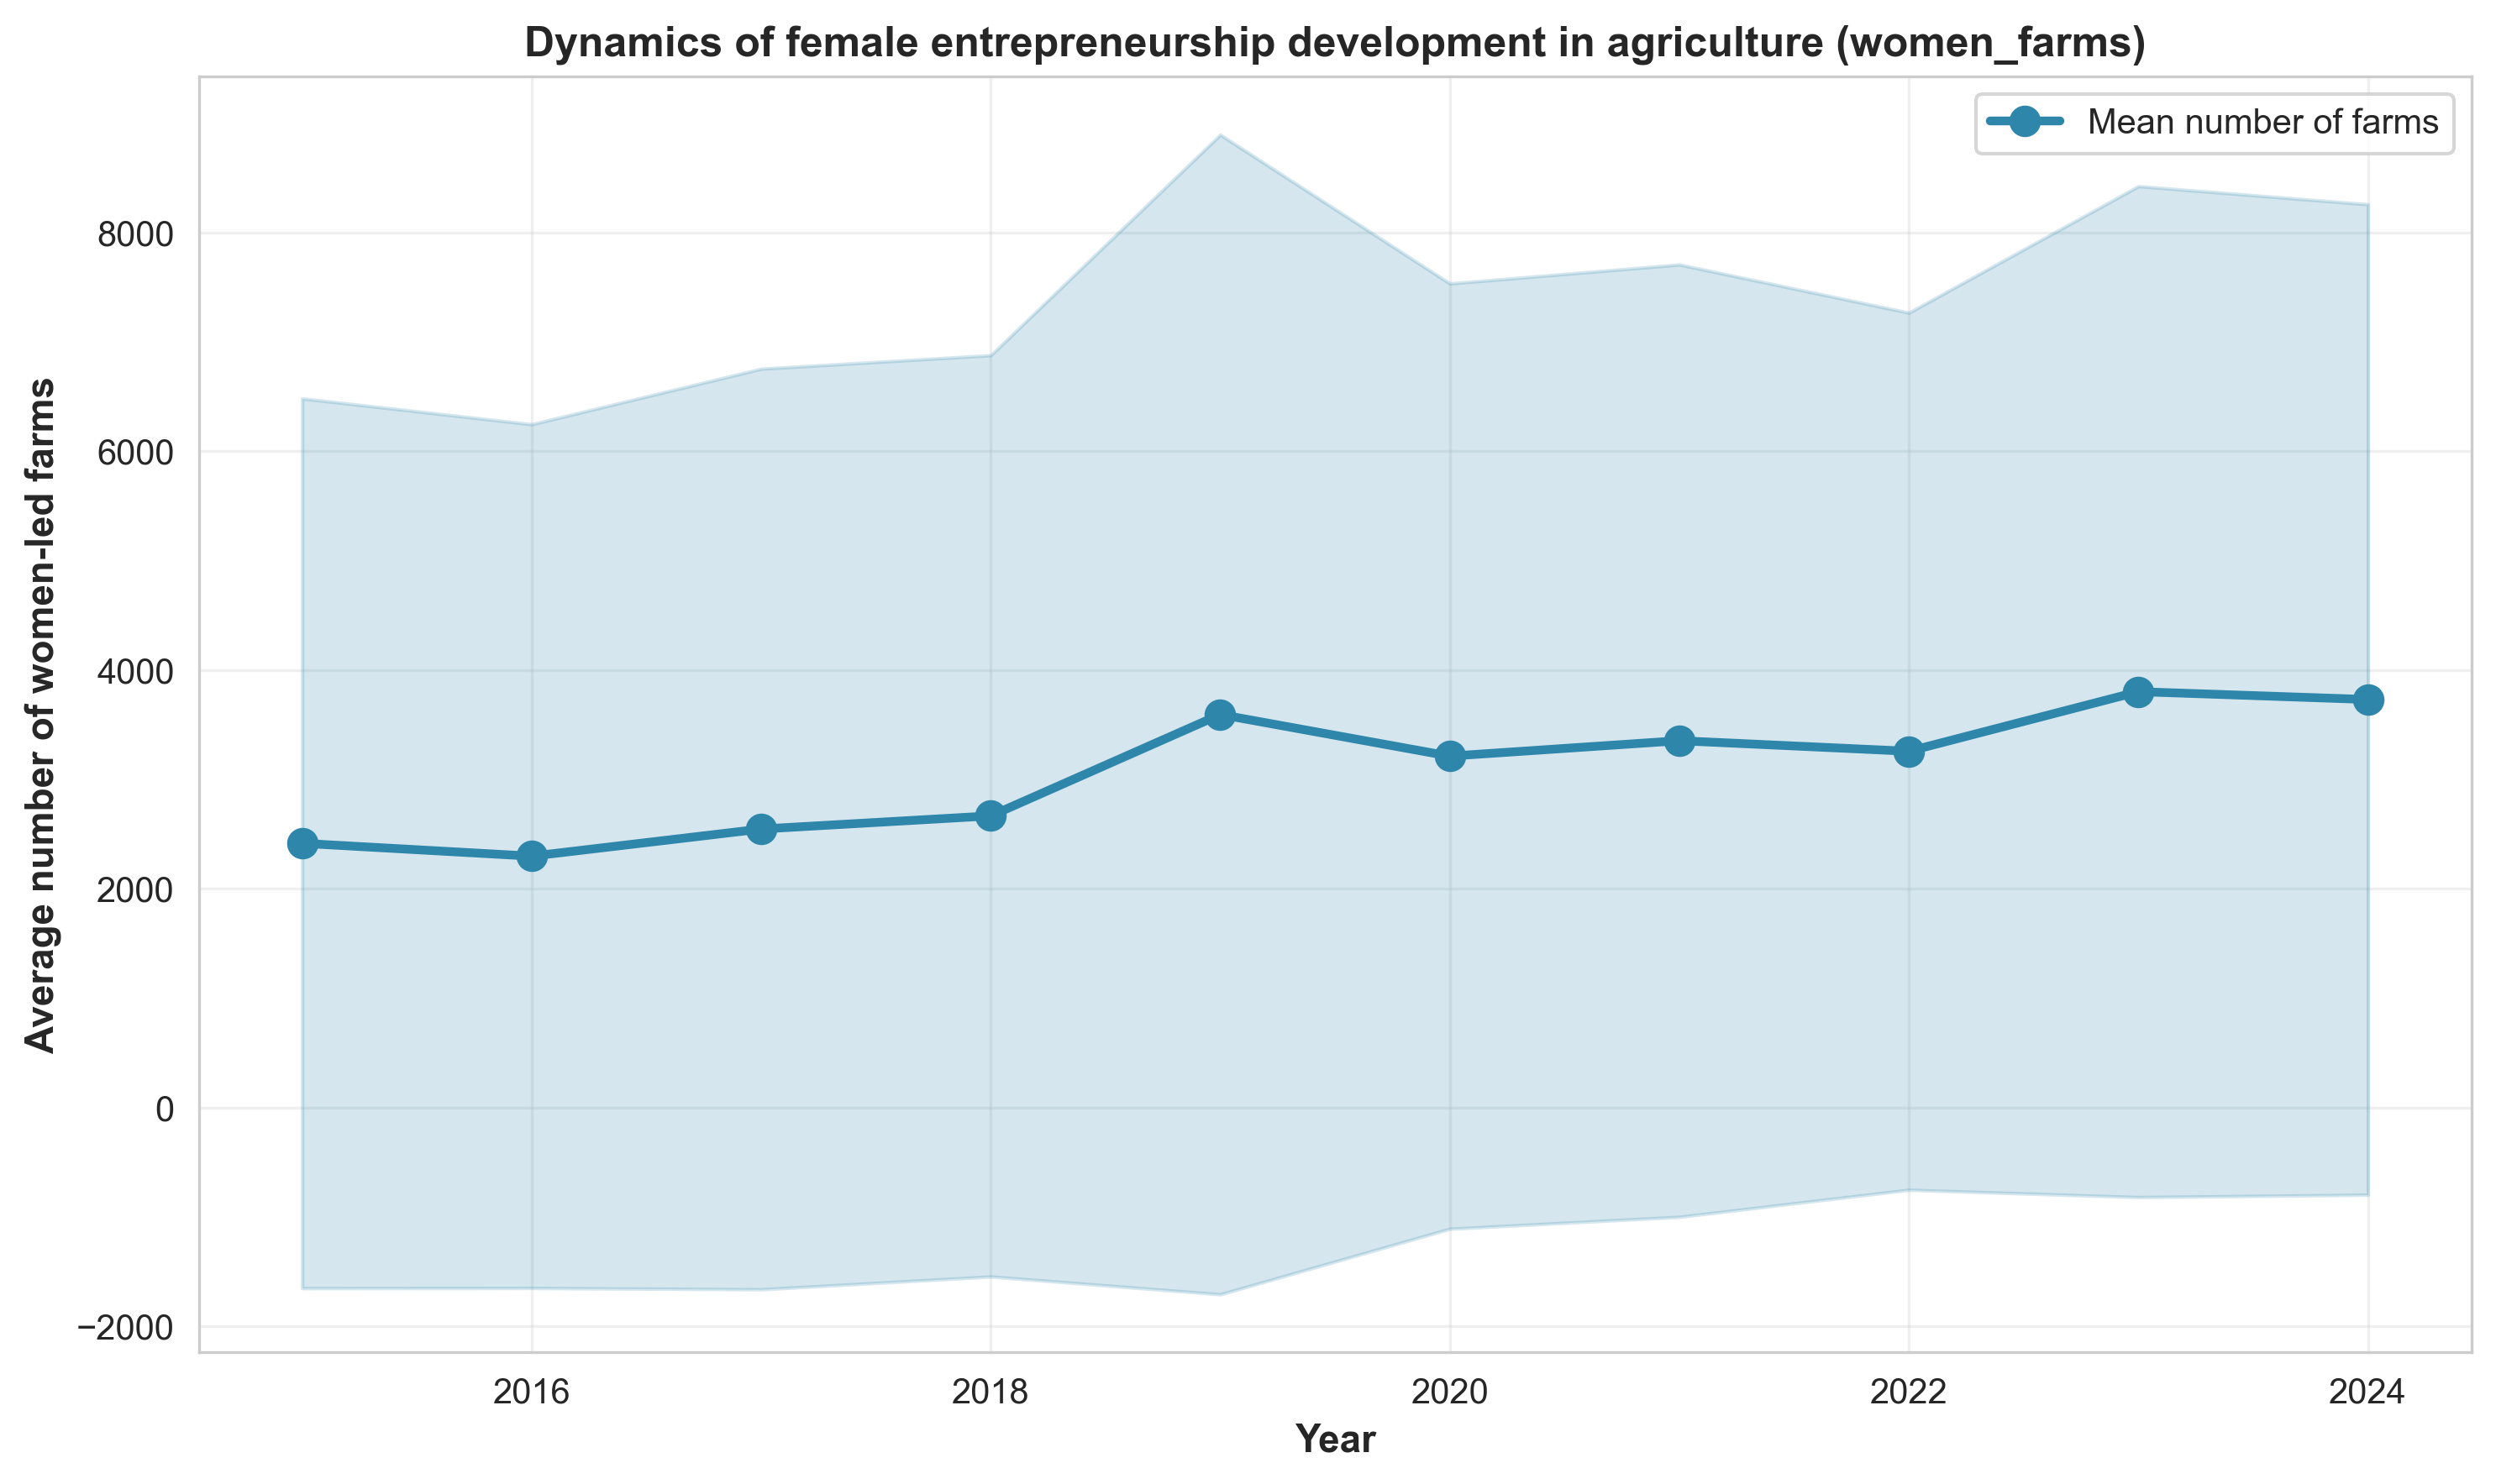
\includegraphics[width=\linewidth,keepaspectratio]{figures/figure02.png}
\caption{Average number of women-owned farms, by region of Kazakhstan, 2015--2024}
\label{fig:women-farms-region}
\end{figure}

Although the volume of loans increased from 3 billion tenges to 4.5
billion tenges, this growth was concentrated in regions with more
developed infrastructure (Figure 2). Econometric analysis confirms this
conclusion. Pooled OLS summary data show a positive correlation between
the number of farms owned by women and the volume of loans. However,
when accounting for regional fixed effects via the TWFE, this correlation
disappears. The main conclusion is that financial institutions such as
Kazagrofinance, the Agrarian Credit Corporation, and the Agricultural
Financial Support Fund focus on supporting developed regions.

\begin{figure}[H]
\centering
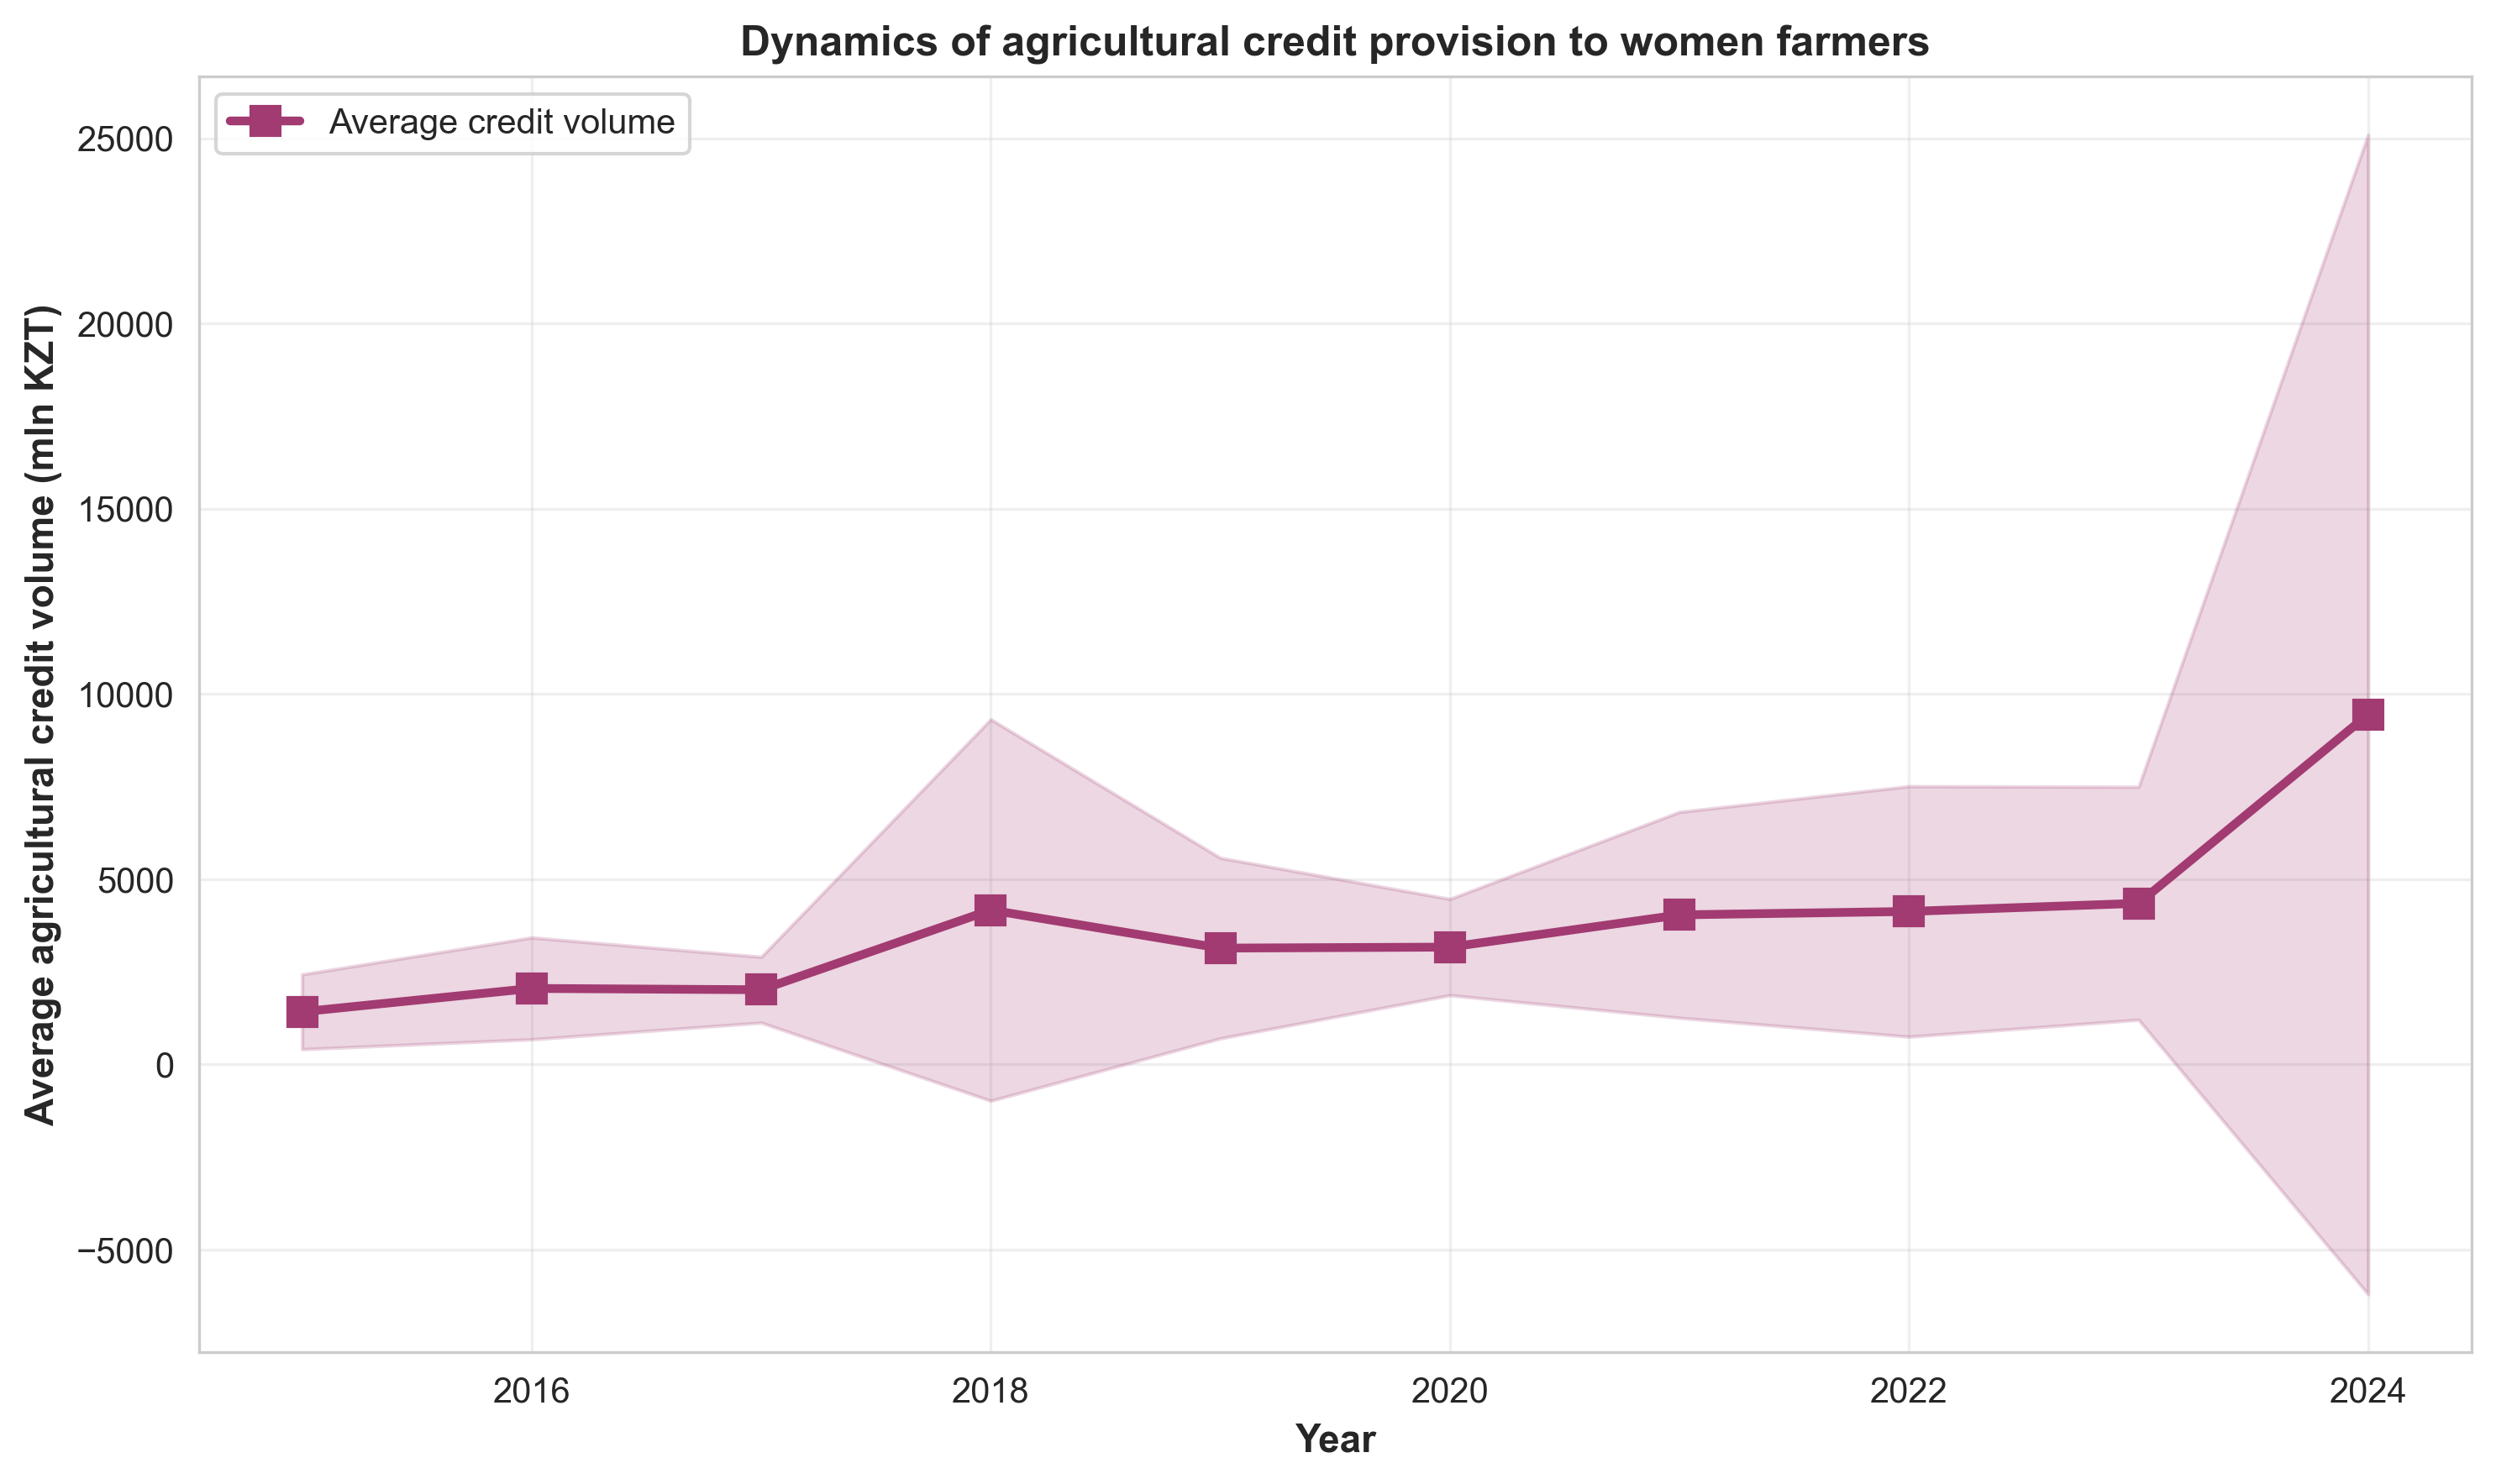
\includegraphics[width=\linewidth,keepaspectratio]{figures/figure03.png}
\caption{Volume of loans issued to women farmers}
\label{fig:loans-volume}
\end{figure}

The scatter plot (Figure 3) shows a significant correlation between the
volume of institutional lending and the number of farms owned by women
(r = 0.576, p \textless{} 0.001). Regions with high levels of lending
are characterized by a large number of farms. Estimation of the two-way
fixed effects (TWFE) model revealed that after accounting for regional
differences, the coefficient of the lending variable decreased from
0.725 to 0.044 and lost statistical significance (p = 0.576). This
implies that lending flows to developed regions but does not stimulate
women's entrepreneurship within those regions. This raises the following
question:
are loans effective, or are there other factors at play?

\begin{figure}[H]
\centering
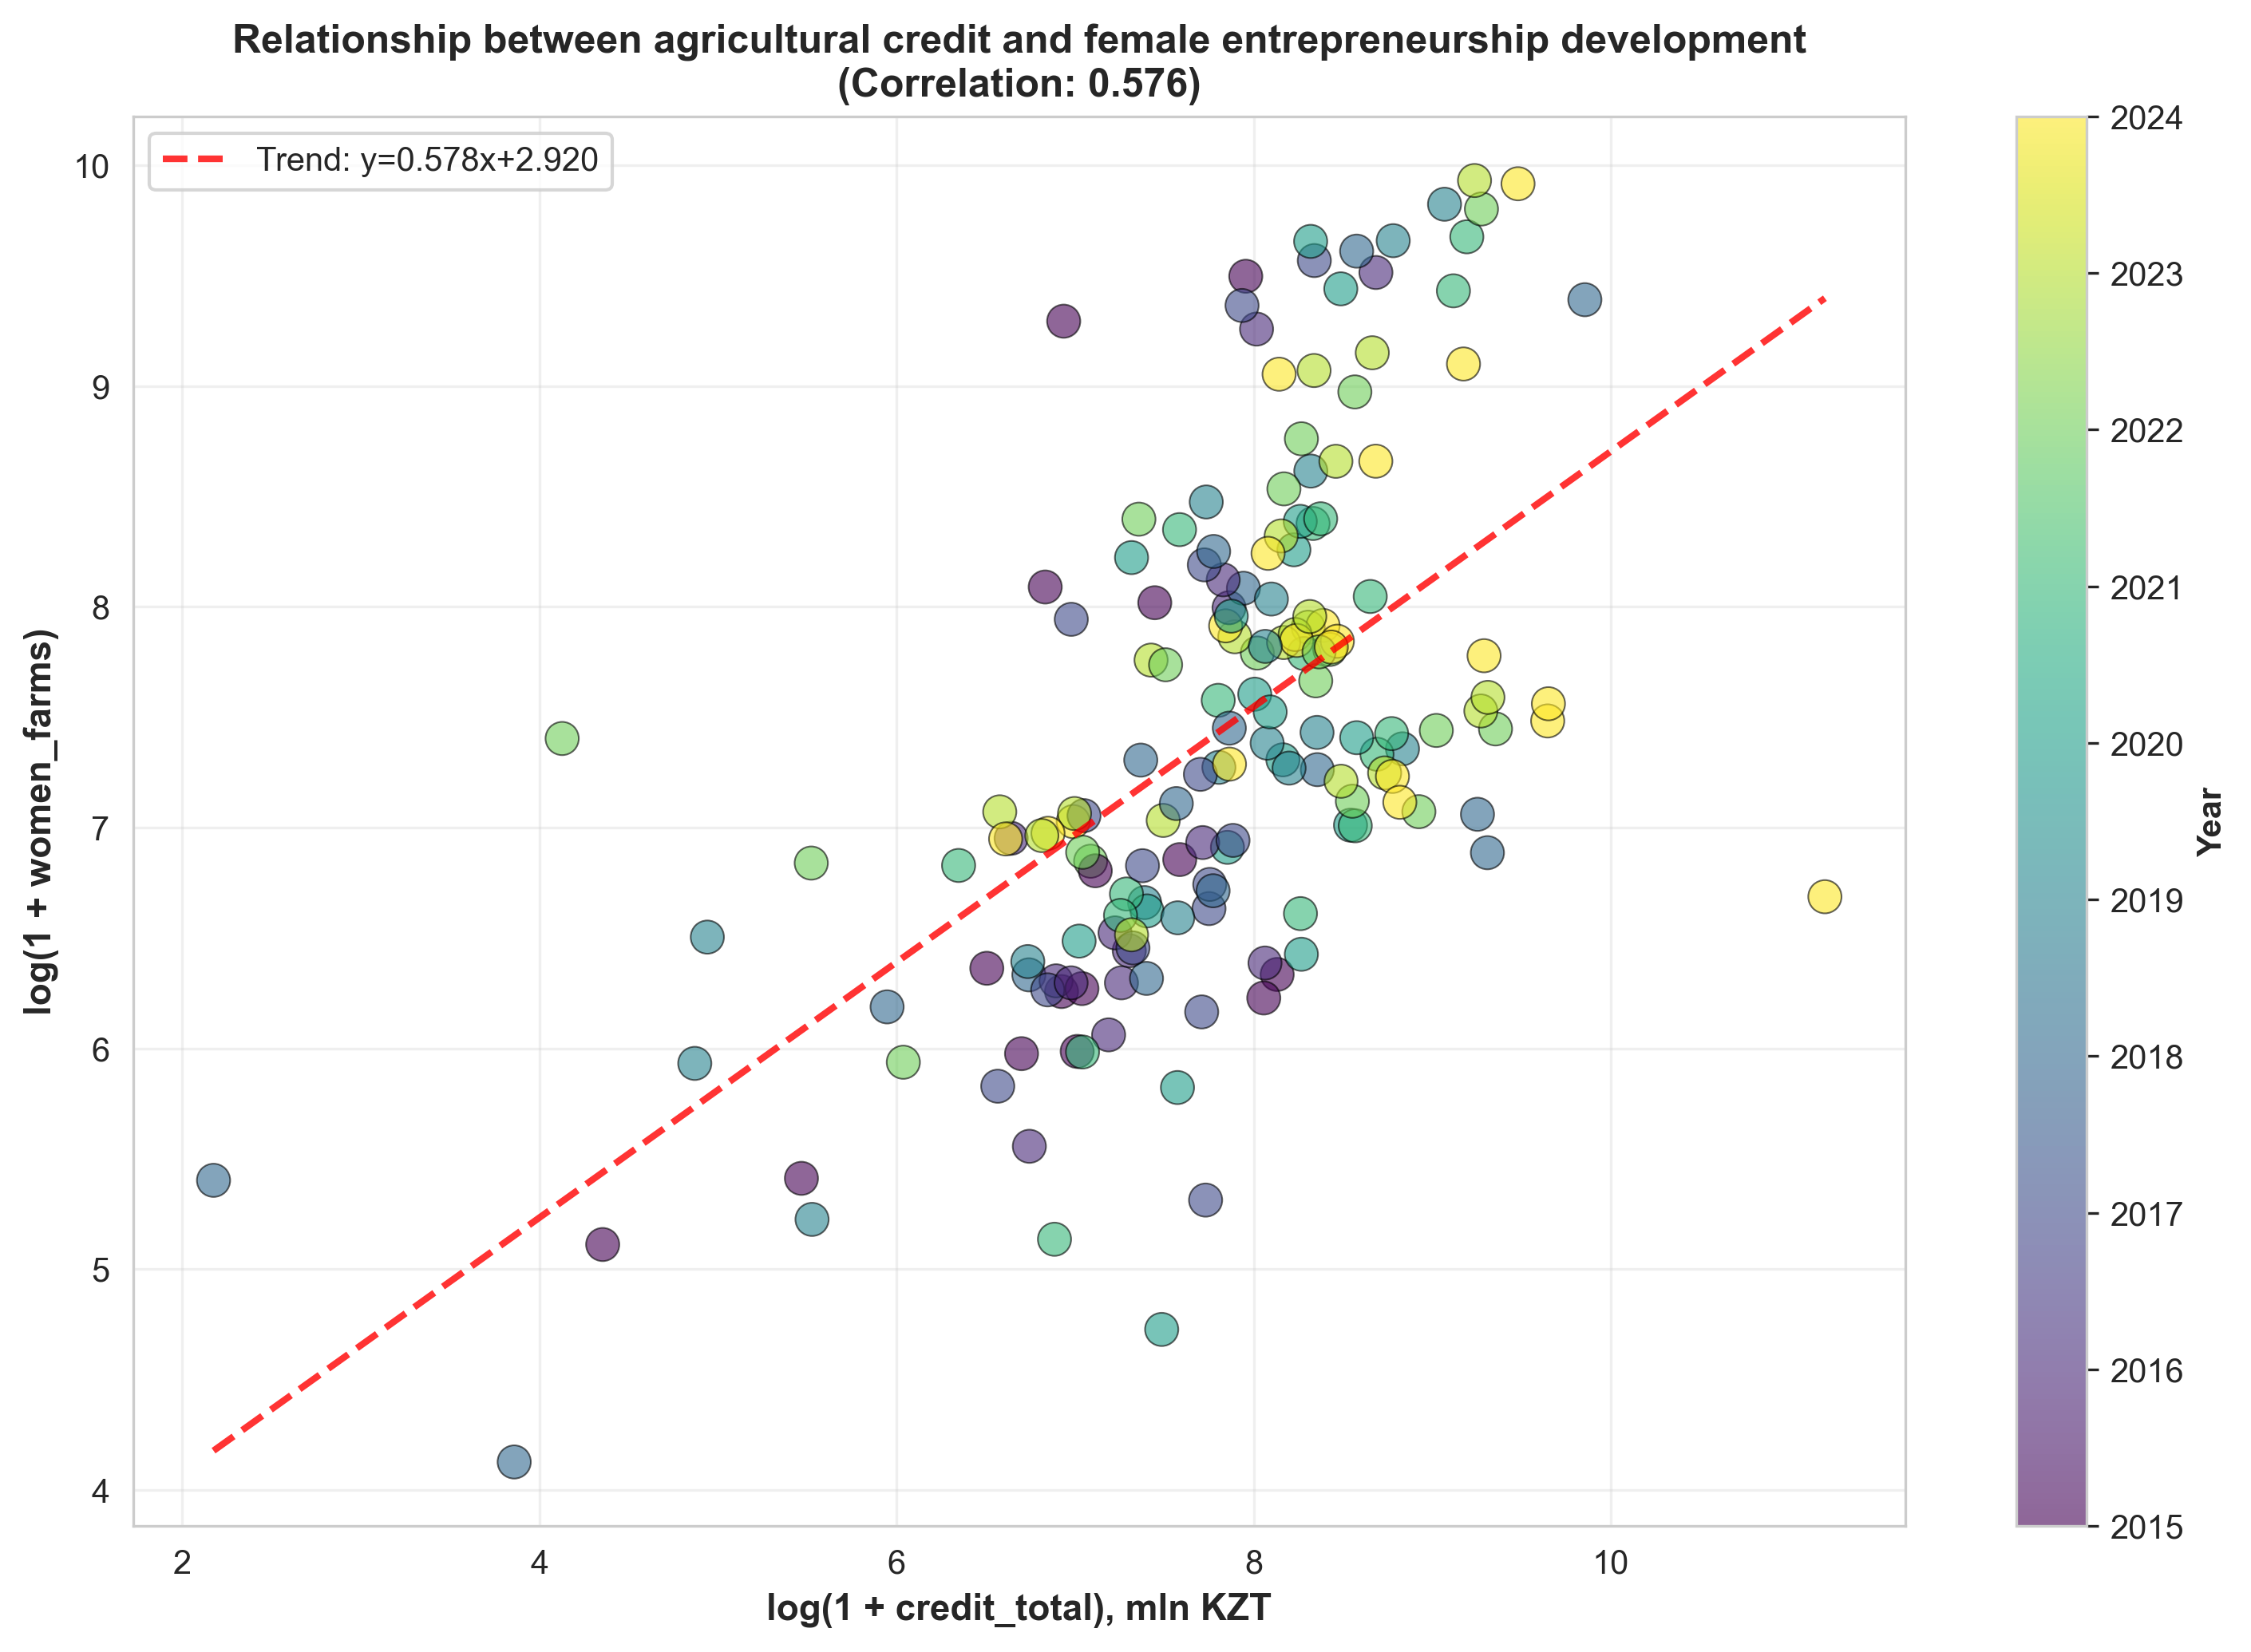
\includegraphics[width=\linewidth,keepaspectratio]{figures/figure04.png}
\caption{The relationship between lending and women's entrepreneurship in agriculture}
\label{fig:lending-entrepreneurship}
\end{figure}

Correlation analysis
alone does not allow us to draw conclusions about the causal nature of
this relationship. The observed relationship may reflect the influence
of third factors, such as the region's level of economic development,
the quality of the institutional environment, or the availability of
infrastructure. In our view, the observed correlation can be explained
by other regional factors or by a feedback mechanism, whereby the growth
of women's entrepreneurship increases the demand for loans.

\subsection{Panel regression results: econometric analysis}

\begin{table}[htbp]
\caption{Comparison of pooled OLS and TWFE}\label{tab:pooled-twfe}
\small
\begin{tabular*}{\textwidth}{@{\extracolsep{\fill}}p{0.26\textwidth}rrrr@{}}
\toprule
Variable & Coefficient & Standard Error & Coefficient & Standard Error\\
 & \multicolumn{2}{c}{Pooled OLS} & \multicolumn{2}{c}{TWFE}\\
\midrule
log\_credit\_total & 0.7250*** & (0.0901) & 0.0443 & (0.0834)\\
land\_share & 0.0566* & (0.0341) & 0.0181 & (0.0289)\\
Constant & 1.7143** & (0.6916) & - & -\\
\midrule
N & 149 &  & 149 & \\
$R^2$ & 0.336 &  & 0.030 (within) & \\
Adjusted $R^2$ & 0.327 &  & 0.099 (overall) & \\
Fixed effects & No &  & Region + Year & \\
SE type & HC1-robust &  & Clustered (region) & \\
\botrule
\end{tabular*}
\end{table}

We constructed a panel regression model to assess the impact of
institutional lending on the development of women-owned farms.

Stage 1: Ordinary least squares (Pooled OLS)

The pooled ordinary least squares (OLS) method revealed a positive
correlation between total credit volume and the number of female-headed
farms. The coefficient for the log\_credit\_total variable was 0.725 (p
\textless{} 0.001). This is explained by the fact that a 1\% increase in
credit leads to a 0.73\% increase in the number of female-headed farms.
$R^2$ = 0.336, meaning that the model explains 33.6\% of the interregional
variation in the dependent variable. The land access variable
land\_share is also significant at the 10\% level, confirming the
importance of land rights for women.

The pooled OLS model revealed that the greater the volume of lending,
the greater the number of farms. However, these regions initially have
better infrastructure and access to loans. In other
words, the specification of this model does not account for these
regional characteristics.

Stage 2. TWFE Fixed-effects model

To account for these differences, we applied the TWFE fixed effects
model, which incorporates these regional characteristics. Here, we
observe that the coefficient for the credit variable decreases from
0.725 to 0.044 and loses statistical significance (p = 0.596).

The following conclusions can be drawn: the second TWFE model primarily
reflects interregional differences, meaning that loans are initially
concentrated in regions with higher levels of women's entrepreneurship
rather than stimulating their growth in regions. This finding further
confirms the hypothesis that financial instruments are unable to
stimulate the growth of women's entrepreneurship without corresponding
institutional reforms, including expanding women's access to land.

\begin{figure}[H]
\centering
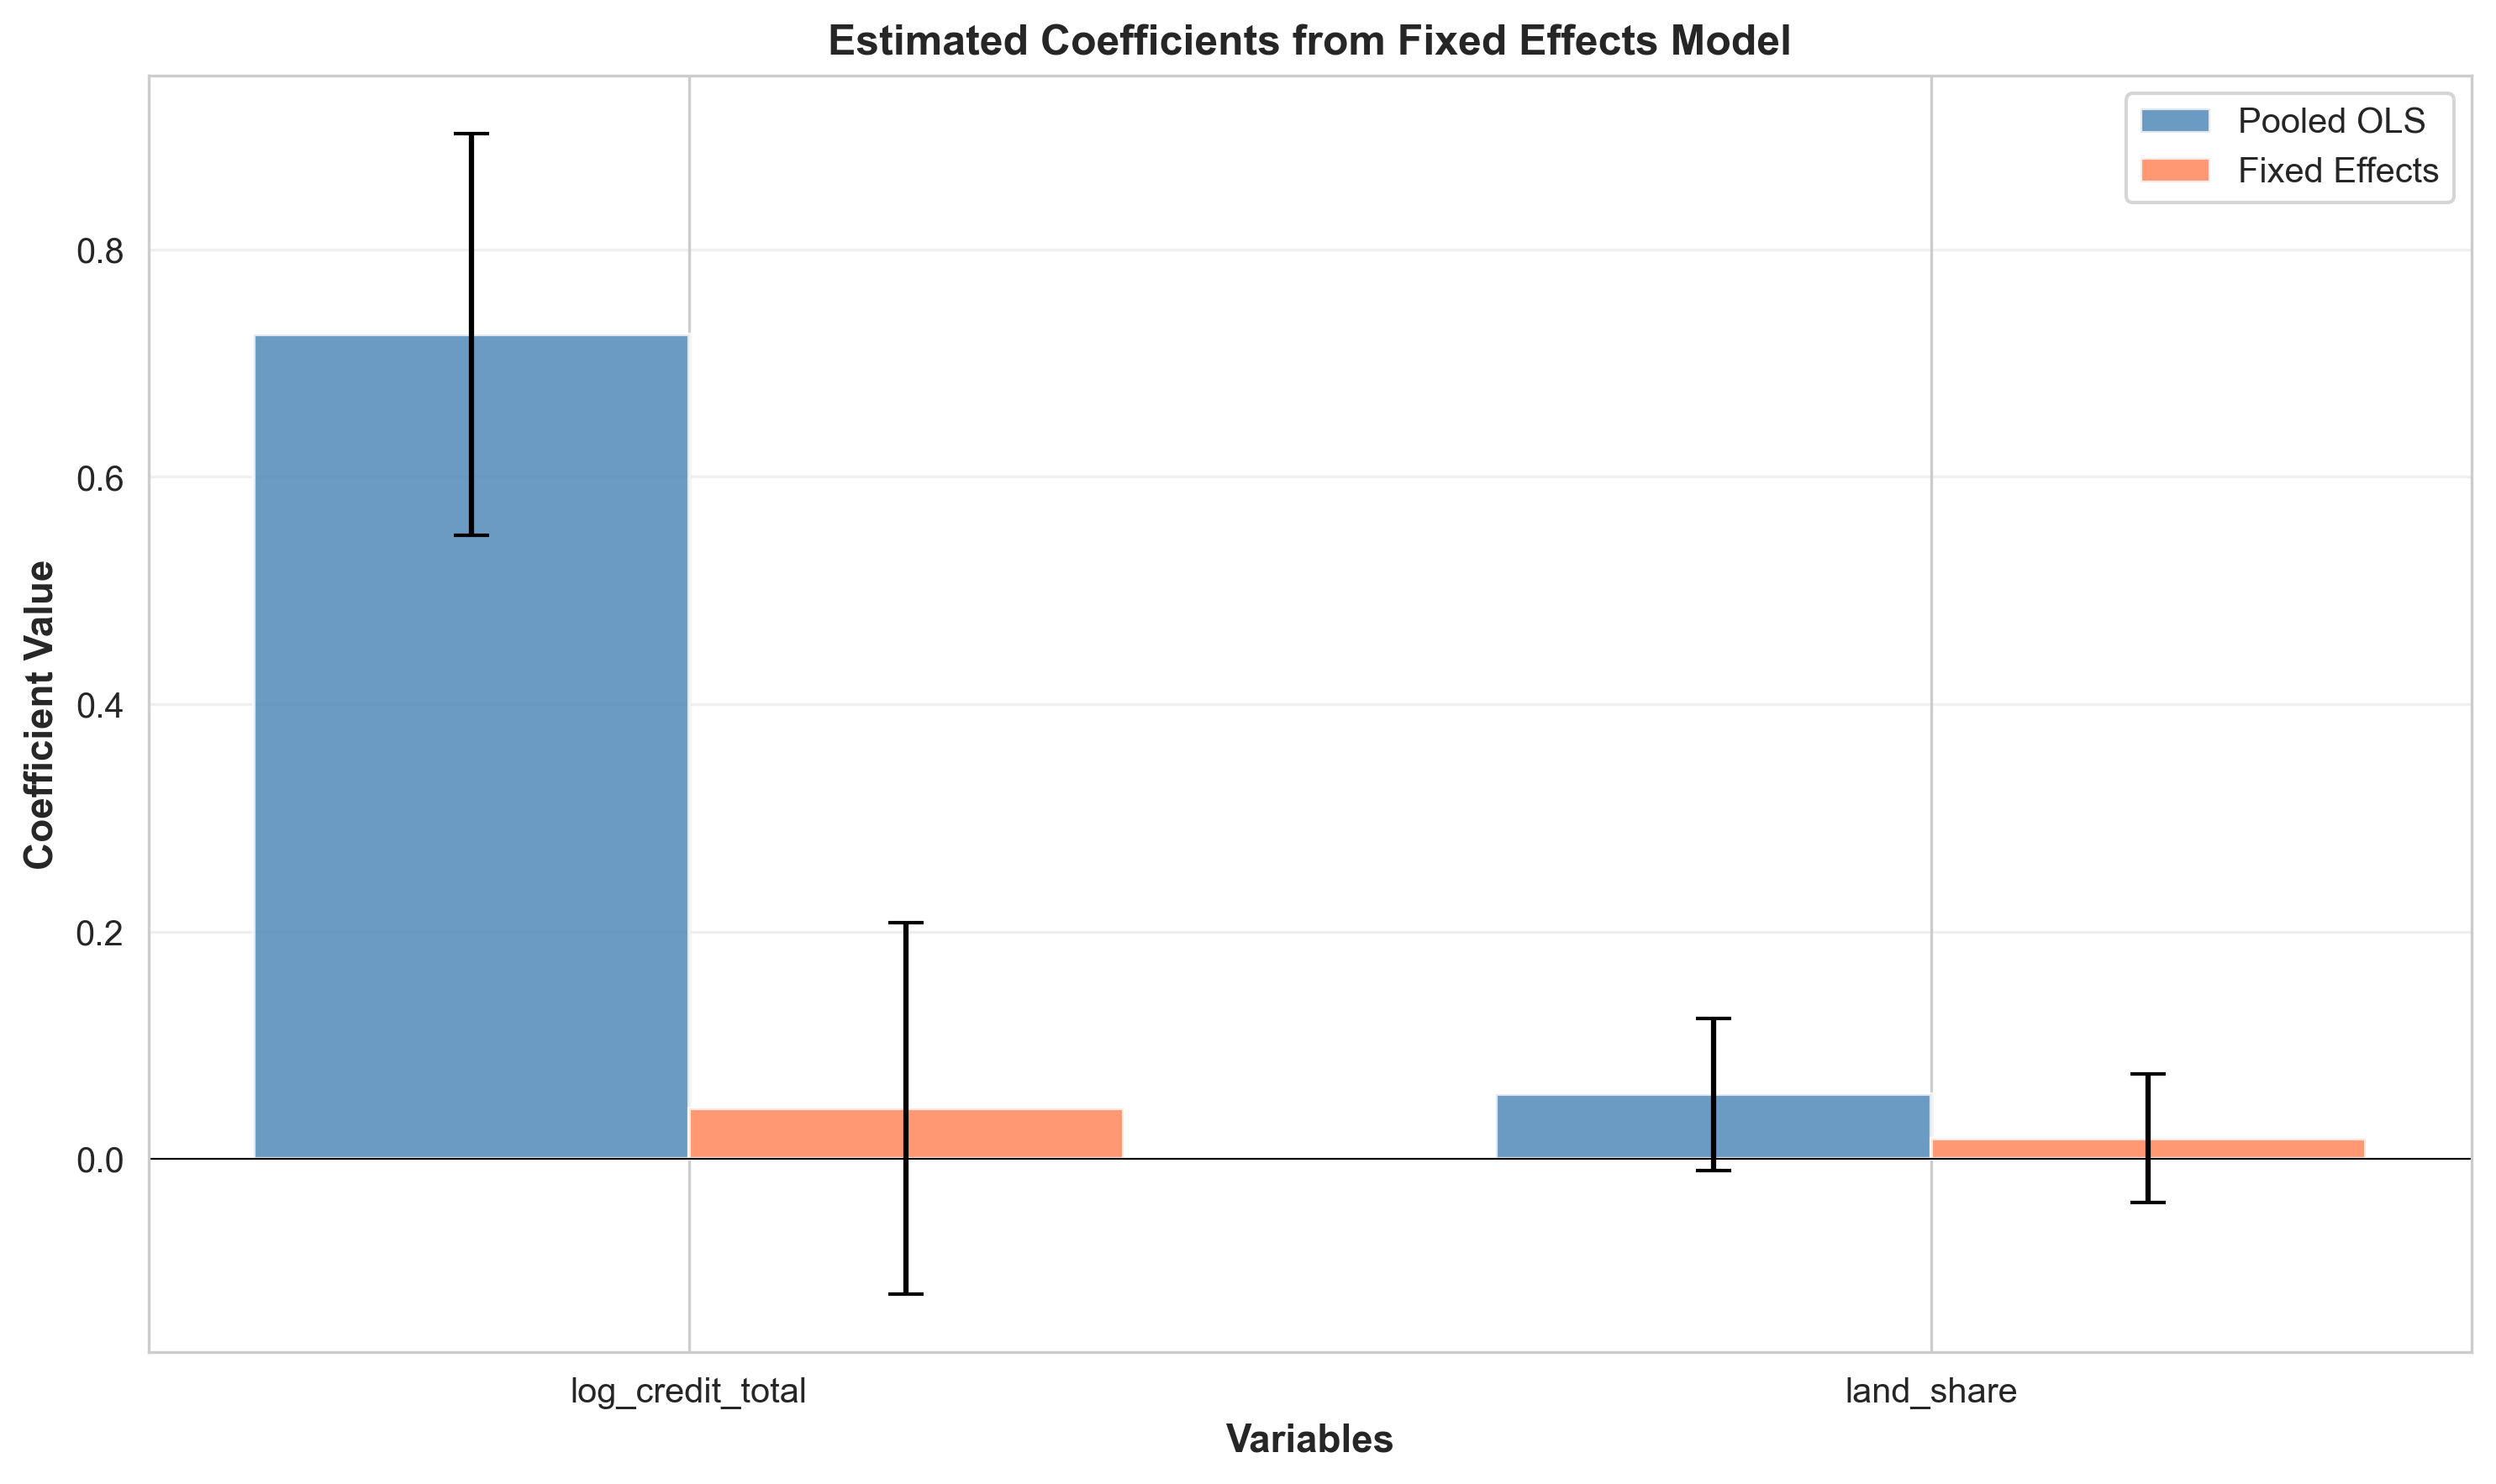
\includegraphics[width=\linewidth,keepaspectratio]{figures/figure05.png}
\caption{Comparison of the pooled OLS and TWFE models}
\label{fig:pooled-vs-twfe}
\end{figure}

Figure 5 clearly shows that in the pooled OLS model, the credit
coefficient is positive at 0.725 (p \textless{} 0.001) and significant.
In the TWFE model, it is practically zero (0.0443) and crosses the zero
line on the graph. This confirms that the observed interregional
correlation is due to interregional differences, rather than the impact
of lending on women's entrepreneurship.

Stability test by decomposing lending into sources

We replaced the aggregate lending indicator with three components: loans
from KazAgroFinance JSC, Agrarian Credit Corporation JSC, and the
Agricultural Financial Support Fund JSC.

\begin{table}[htbp]
\caption{Results of the model estimation by lending source}\label{tab:lending-source}%
\small
\begin{tabular*}{\textwidth}{@{\extracolsep{\fill}}p{0.28\textwidth}rrrrr@{}}
	oprule
Variable & Coefficient & Standard error & t-statistic & p-value & N\\
\midrule
log\_credit\_kaf & 0.0031 & (0.0365) & 0.084 & 0.933 & 88\\
log\_credit\_acc & -0.0473 & (0.0484) & -0.979 & 0.331 & 88\\
log\_credit\_fund & -0.0073 & (0.0647) & -0.113 & 0.910 & 88\\
\bottomrule
\end{tabular*}
\end{table}

The calculations presented in Table 3 show that none of the three
sources of lending had a statistically significant effect, while the
sample size was reduced to 88 observations because of missing lending
data from the Agricultural Financial Support Fund. The coefficients are
close to zero, ranging from -0.473-/-0.003, and the p values exceed
0.05 (0.933, 0.331, and 0.910). These calculations demonstrated once
again that credit flows do not influence the formation of female-headed
households (data from the main TWFE model).

\subsection{Regional clustering}

To identify regional heterogeneity in the characteristics of women's
entrepreneurship development, the k-means clustering method was applied.
On the basis of seven indicators --- the mean values and standard
deviations of the number of women-owned farms and the volume of lending,
the share of land, and the development trend --- regions were grouped into
two clusters (optimality determined by the silhouette score criterion =
0.400) (Table 4).

\begin{table}[htbp]
\caption{Regional cluster profiles}\label{tab:cluster-profiles}
\scriptsize
\renewcommand{\arraystretch}{1.1}
\setlength{\tabcolsep}{3pt}
\begin{tabularx}{\textwidth}{>{\raggedright\arraybackslash}p{0.12\textwidth}>{\centering\arraybackslash}p{0.11\textwidth}>{\raggedright\arraybackslash}X>{\raggedright\arraybackslash}X>{\raggedright\arraybackslash}X>{\centering\arraybackslash}p{0.12\textwidth}}
\toprule
Cluster & Number of regions & \shortstack[l]{log\_women\_farms\\(mean)} & \shortstack[l]{log\_credit\_total\\(mean)} & Share of land (average, \%) & Growth trend (annual)\\
\midrule
Cluster 0 & 15 & 7.71 & 8.02 & 2.30 & 0.091\\
Cluster 1 & 5 & 6.35 & 6.75 & 0.18 & 0.296\\
\botrule
\end{tabularx}
\setlength{\tabcolsep}{6pt}
\renewcommand{\arraystretch}{1}
\end{table}

\emph{Note:} Average characteristics of regional clusters. Growth trend -- the
slope of the log\_women\_farms linear trend over time, characterizing
the growth rate of women's entrepreneurship. *

The cluster analysis divided the regions into two groups.

Cluster 0 (15 regions) includes rural areas with a high level of women's
farming (log\_women\_farms = 7.71, corresponding to approximately 2,230
farms on average per region), high total credit volume
(log\_credit\_total = 8.02, or approximately 3,050 million tenge), and a
relatively high share of land owned by women (2.30\%). However, the
growth rate here is moderate: 0.091 logarithms per year, which
translates to approximately 9.5\% annual growth.

Cluster 1 (5 regions) -- regions with a low starting point. Here, there
are four times fewer women-owned farms (log\_women\_farms = 6.35, approximately
570 farms), 3.6 times fewer loans (log\_credit\_total = 6.75, approximately 850
million tenge), and the share of land owned by women is practically zero
(0.18\%). However, the growth rate is three times higher: 0.296
logarithms per year, or approximately 34.5\% growth per year.

\emph{*Note: Since the dependent variable is taken as a natural
logarithm,
the linear trend coefficient $\beta$ corresponds to the approximate growth
rate in percentage terms. For Cluster 0, $\beta$ = 0.091 yields approximately 9.5\%
growth per year; for Cluster 1, $\beta$ = 0.296 yields approximately 34.5\% per
year. *}

According to our calculations, these results are significant for two
reasons. First, rapid growth in regions with low levels of lending
suggests that loans are not the driving force. The dynamics of women's
farming are not determined by the current volume of loans or the
availability of land. Regions with the fewest initial opportunities
demonstrate the greatest growth potential, whereas more developed
regions experience a saturation effect.

The results are consistent with the findings of the fixed-effects
models.

\begin{figure}[H]
\centering
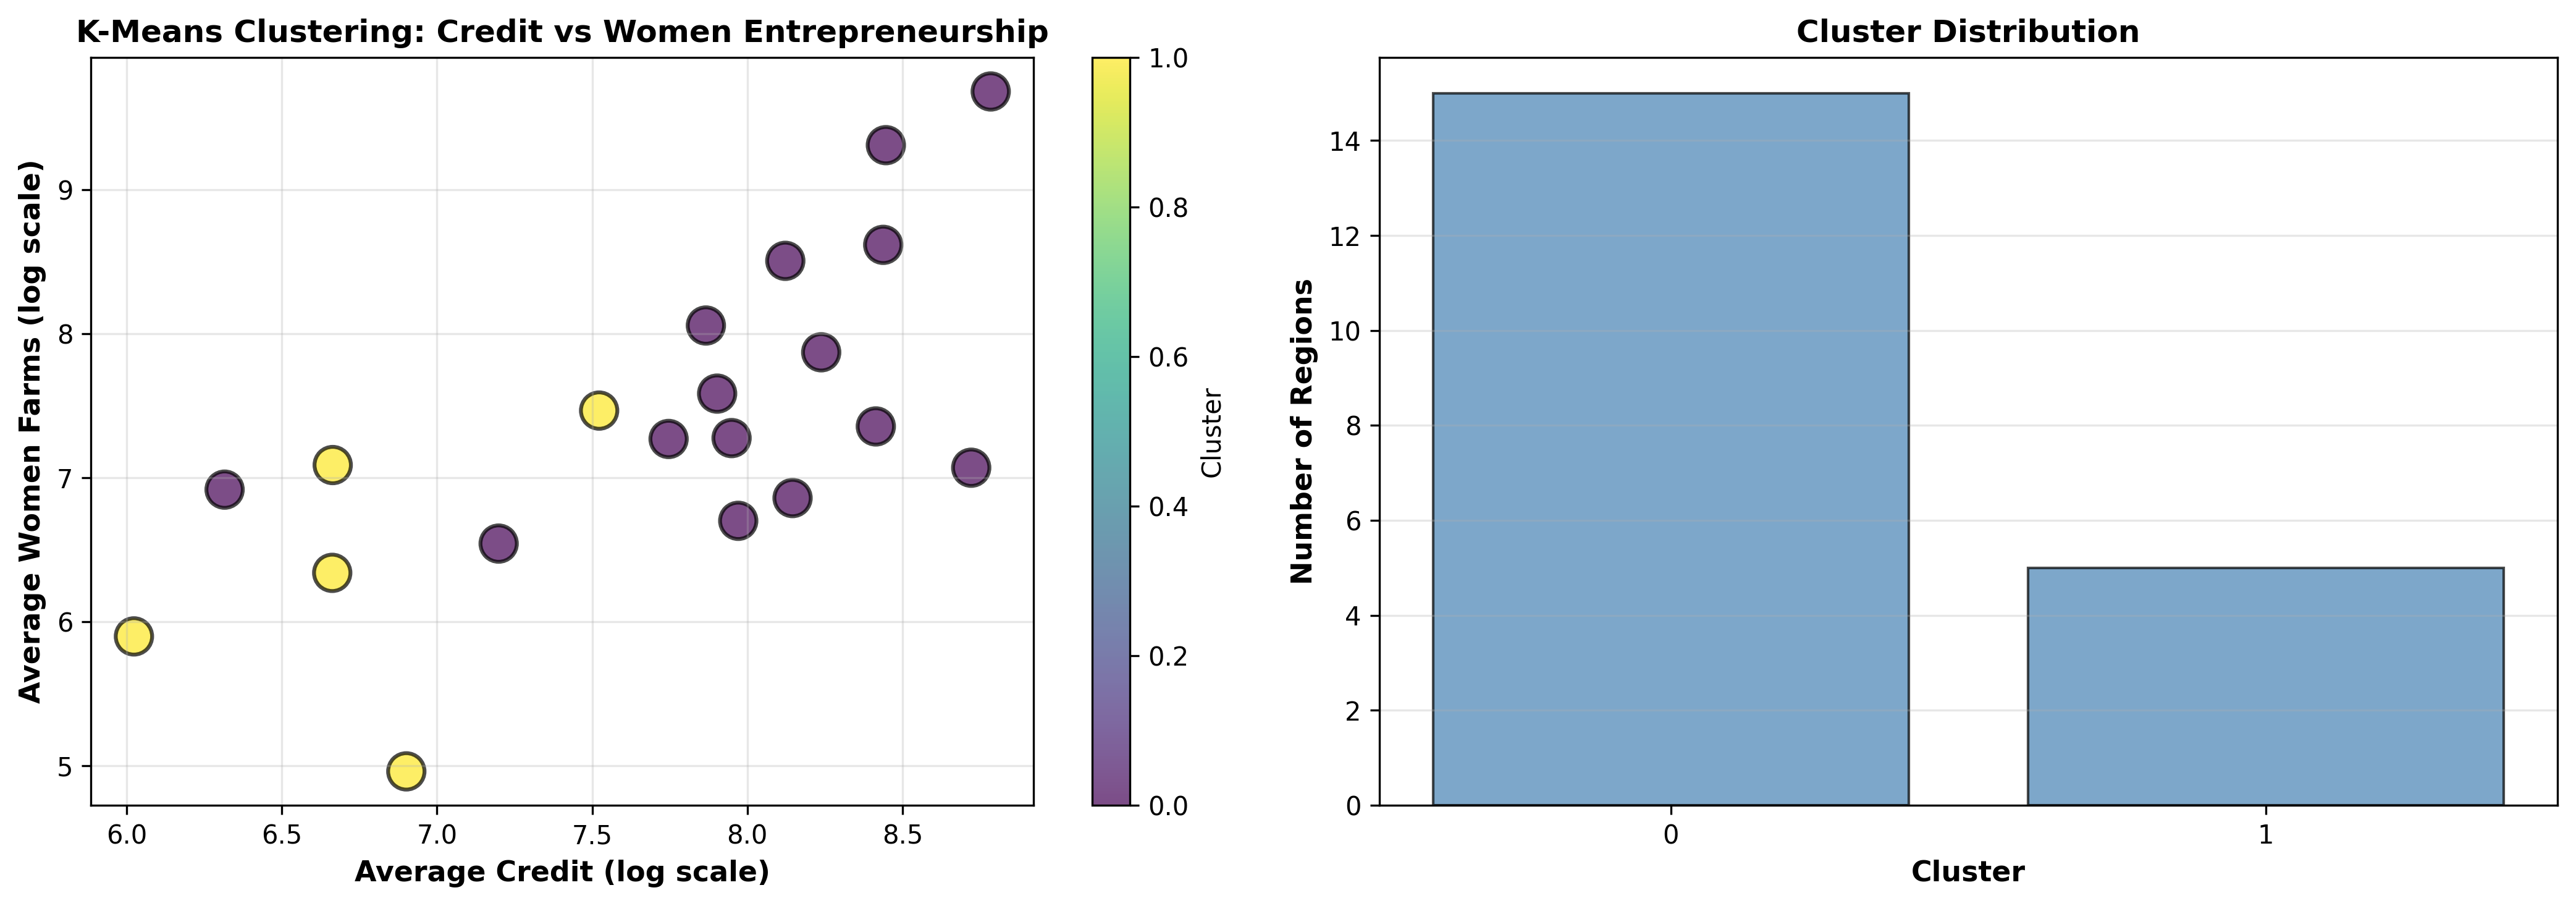
\includegraphics[width=\linewidth,keepaspectratio]{figures/figure06.png}
\caption{Regional clusters based on lending and women's entrepreneurship}
\label{fig:regional-clusters}
\end{figure}

In the scatter
plot, Cluster 0 (blue) is located in the high-value area
along both the lending axis and the women's entrepreneurship axis,
whereas
Cluster 1 (yellow) is in the lower-value area for both characteristics.
Regions with a low baseline but high growth potential (cluster 1)
require different measures than regions where the women's agribusiness
sector has already developed (cluster 0). In our opinion, for the first
group of regions in Kazakhstan, the priority may be the removal of
institutional barriers (access to land and infrastructure), whereas for
the second group, the priority may be improving efficiency and
diversification.

\subsection{Analysis of feature importance: random forest}

To understand which variables best influence the development of women's
farming and to check for nonlinear relationships, we used the random
forest method. The model was trained via group cross-validation
(GroupKFold, 5 folds per region). This ensures that data from the same
region are not included in both the training and test sets.
\begin{table}[htbp]
\caption{Importance of Features from the Random Forest Model}\label{tab:feature-importance}%
\small
\begin{tabular*}{\textwidth}{@{\extracolsep{\fill}}p{0.46\textwidth}rr@{}}
	oprule
Feature & Importance & \% Total\\
\midrule
log\_credit\_fund & 0.448 & 44.76\%\\
log\_credit\_total & 0.146 & 14.56\%\\
log\_credit\_acc & 0.102 & 10.23\%\\
lag1\_log\_credit\_total & 0.102 & 10.22\%\\
land\_share & 0.088 & 8.84\%\\
log\_credit\_kaf & 0.082 & 8.19\%\\
year & 0.032 & 3.20\%\\
\botrule
\end{tabular*}
\end{table}

We used a random forest model to identify the variables that best
predict the development of women's agriculture and to test for nonlinear
relationships that are not detected by linear models. We also used group
cross-validation to assess the model's quality.

The data in Table 5 show that loans provided through the Agricultural
Financial Support Fund account for the largest share at 44.8\%. Total
loans rank second at 14.6\%, nearly three times smaller. This
demonstrates the importance of the funding source and that not all loans
are effective. It is crucial to distinguish loans by source; that is,
the effectiveness of loans is determined by the source, not the volume.
Systematic changes over the years do not affect the dependent variable.
Land is also important for the sustainable development of agriculture
and women's entrepreneurship (8.84\%).

The random forest model showed that the variables can accurately predict
outcomes and confirms a significant correlation between loans and female
farmers. The TWFE model, on the other hand, estimates the change in the
outcome when each factor changes. This suggests that loans are
concentrated in areas where women's entrepreneurship has already
developed. This distinction between correlation and causation is the
result of our study.

\begin{figure}[H]
\centering
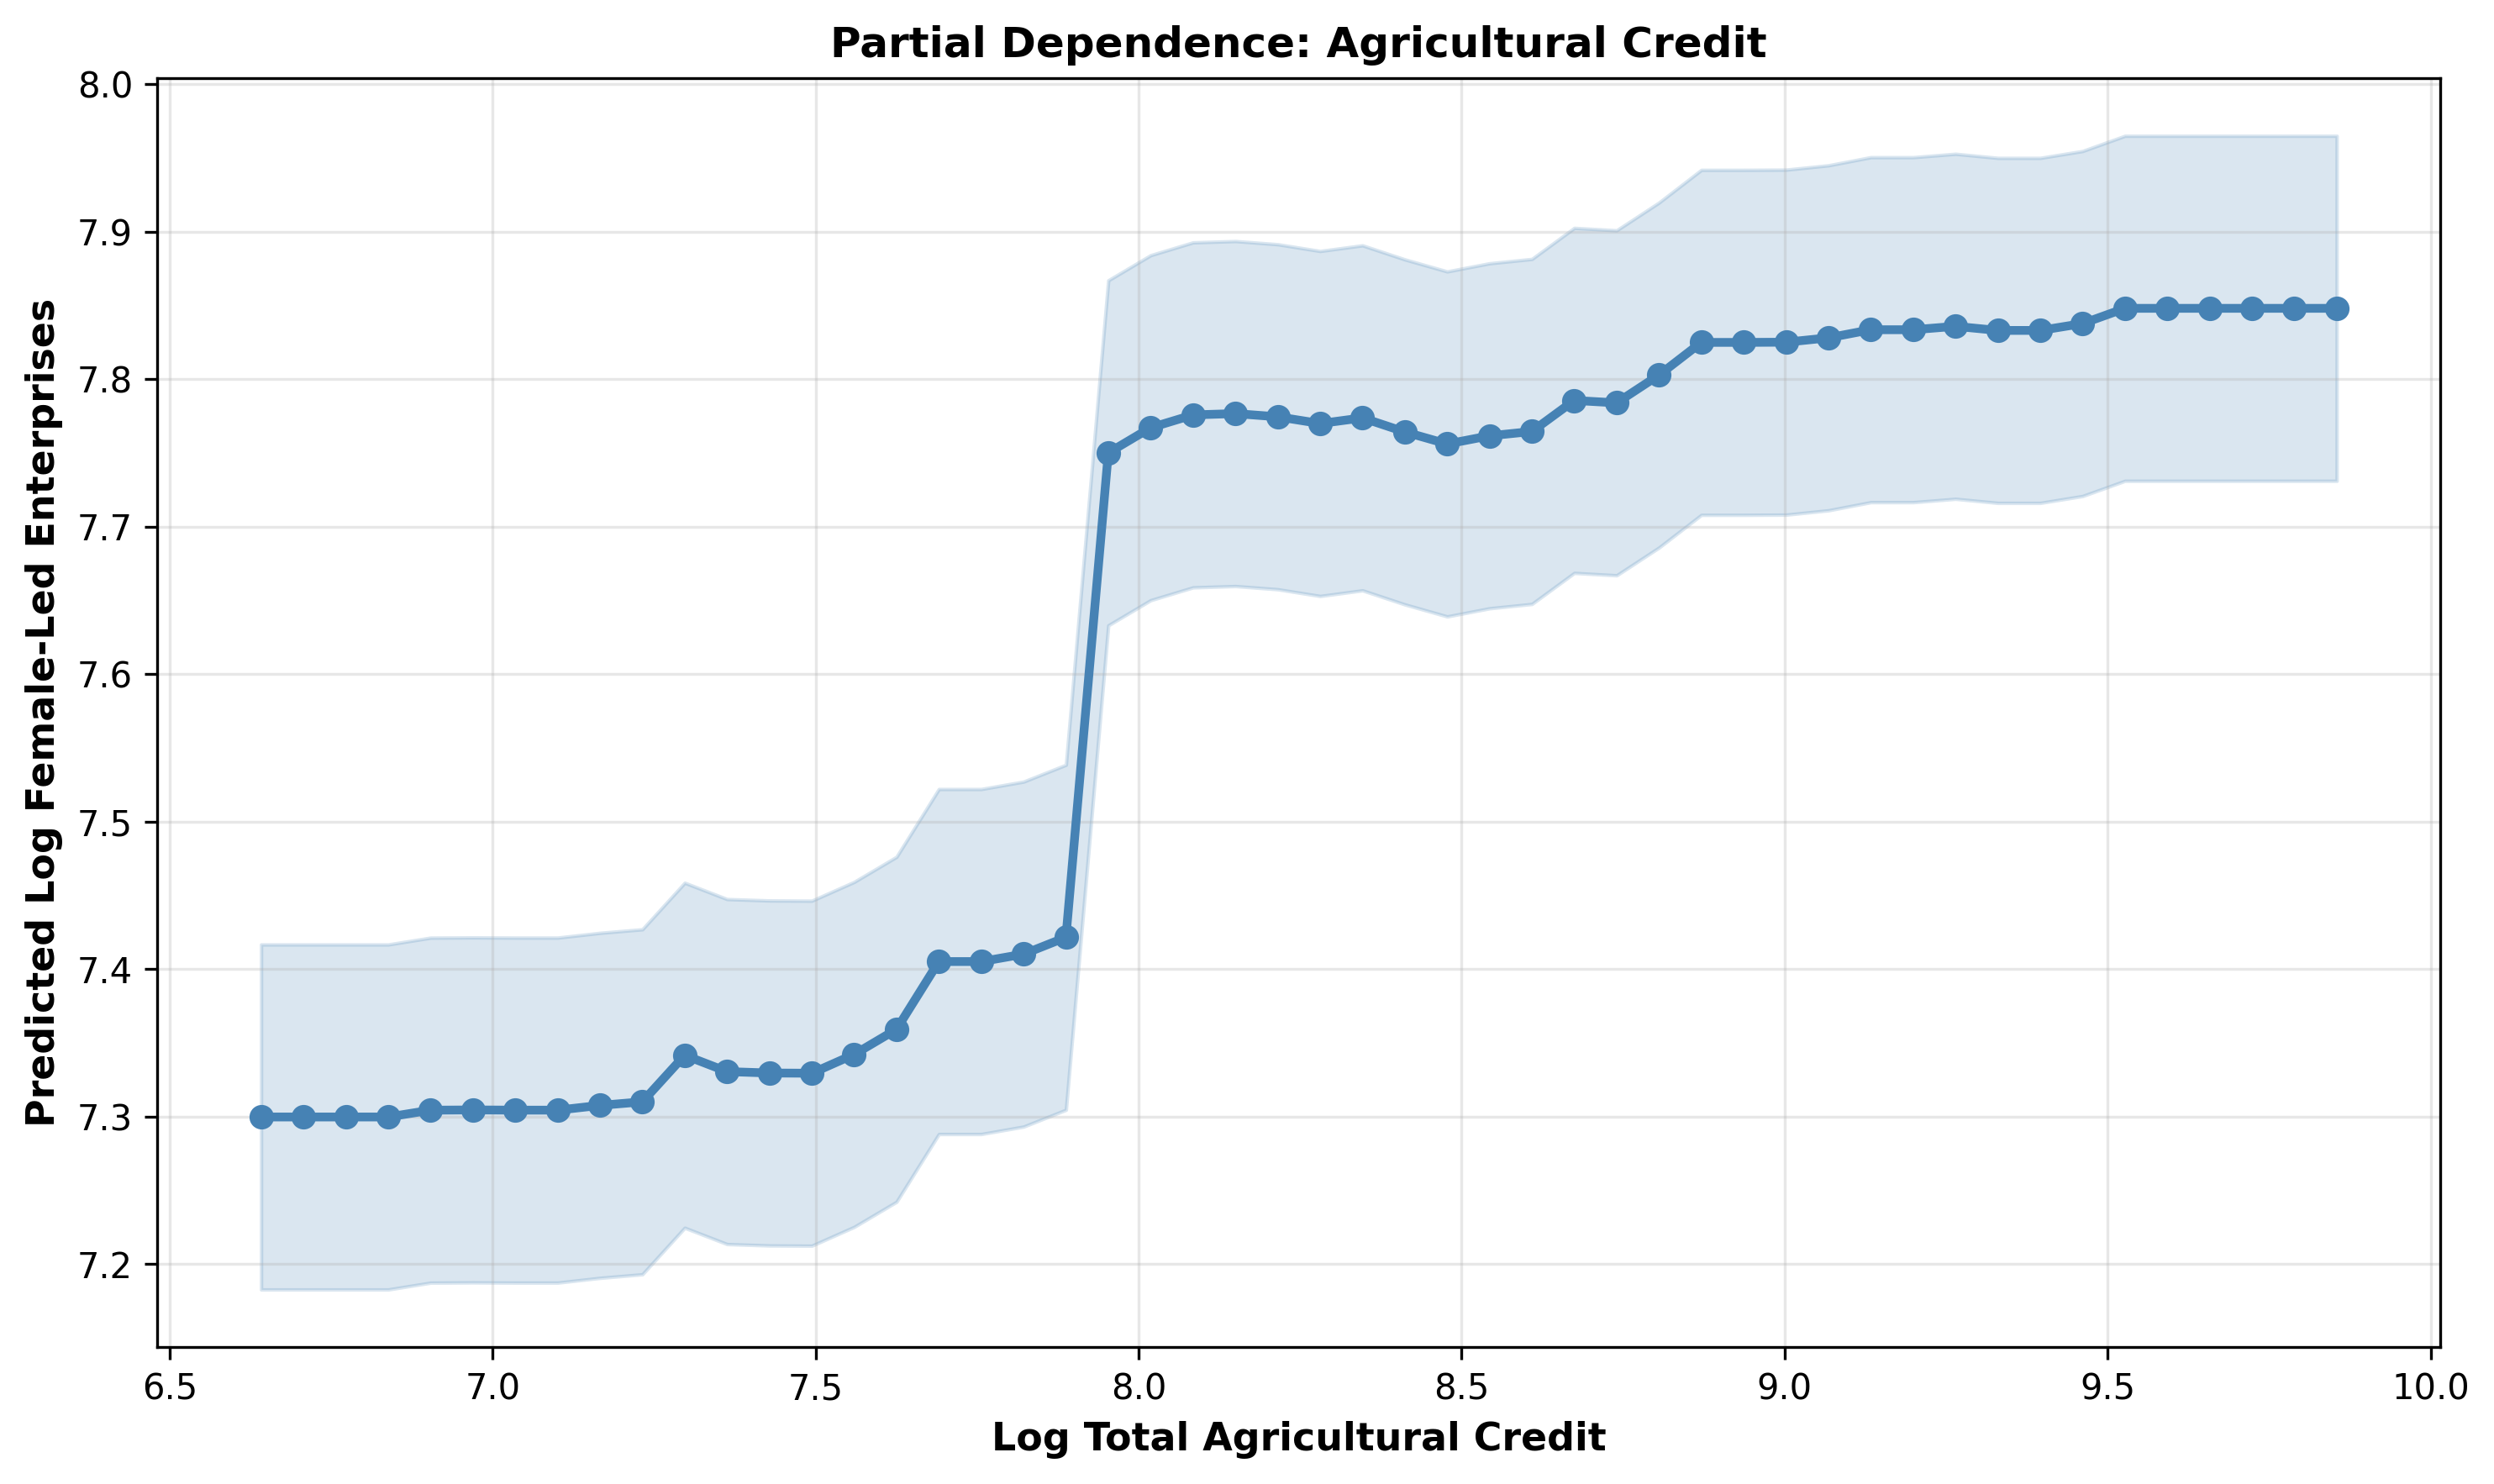
\includegraphics[width=\linewidth,keepaspectratio]{figures/figure07.png}
\caption{Relationship between loan amount and the number of farms owned by women}
\label{fig:loan-amount-farms}
\end{figure}

The graph generated via the random forest model (Figure 7) reveals a
positive correlation between the loan amount and the predicted number of
farms owned by women. The absence of a significant effect in the TWFE
model indicates that the relationship observed in Figure 7 is driven by
the structural characteristics of the regions rather than a causal
effect of loans.

\begin{figure}[H]
\centering
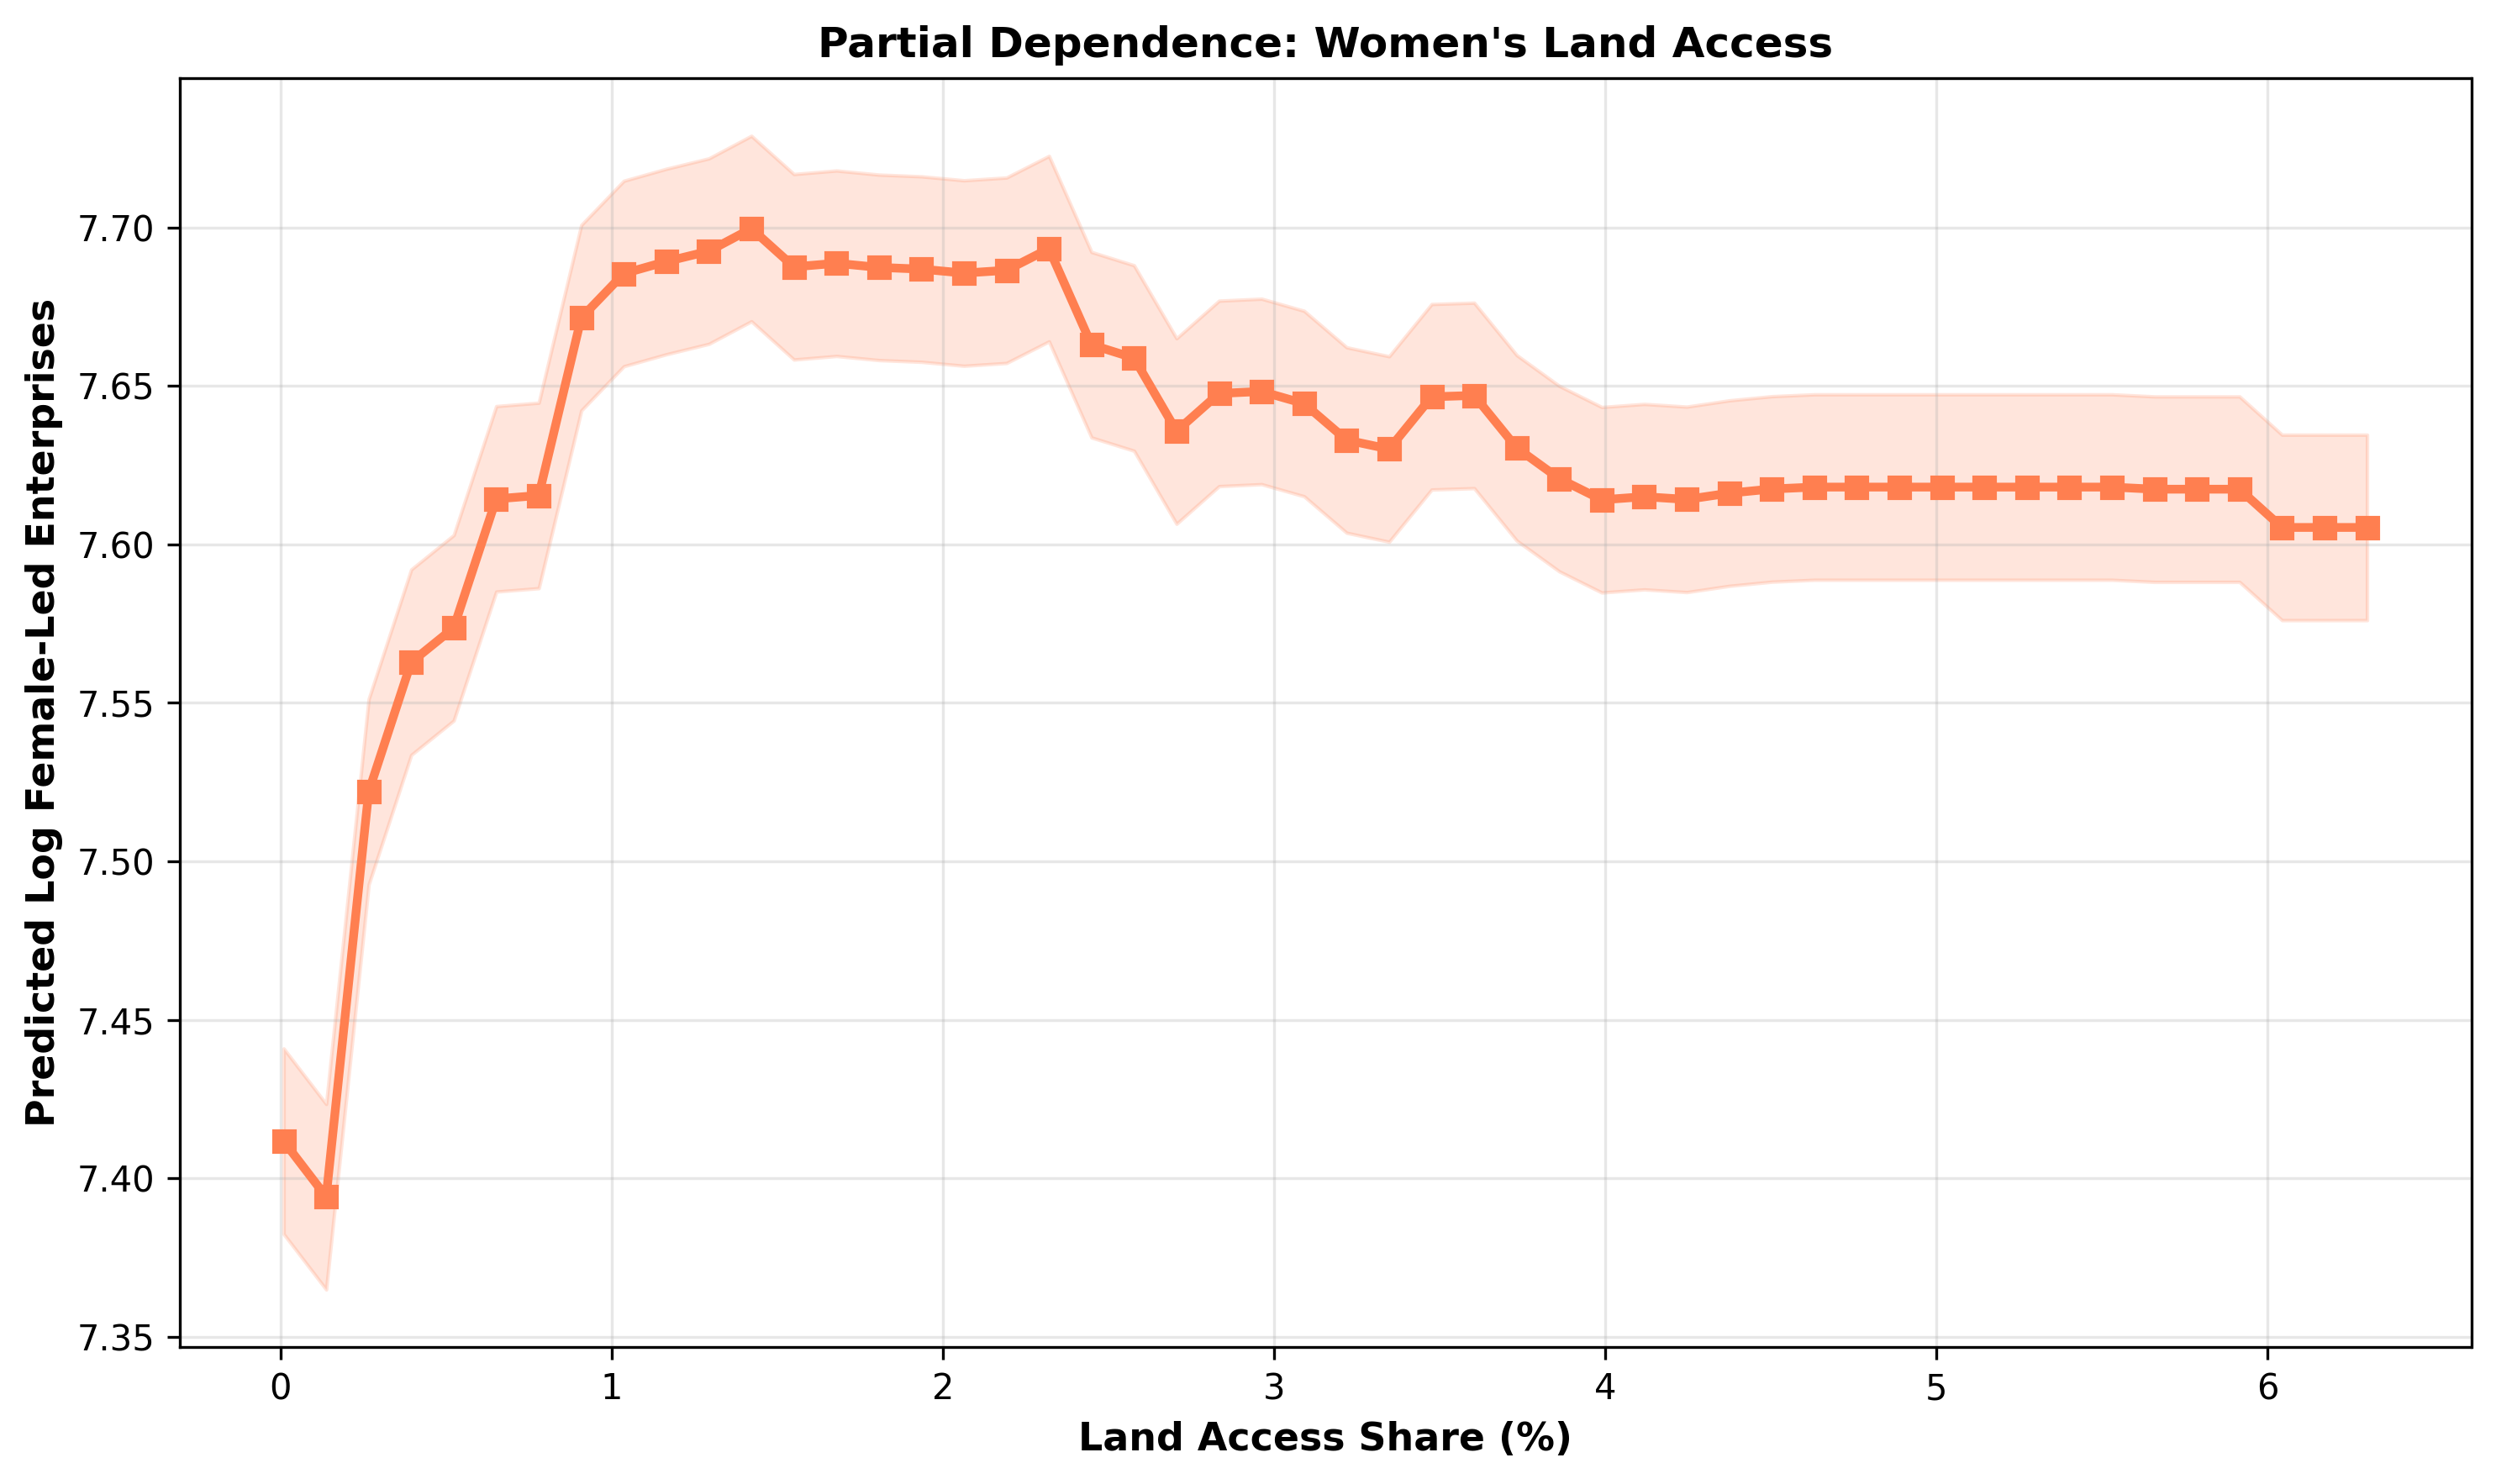
\includegraphics[width=\linewidth,keepaspectratio]{figures/figure08.png}
\caption{Relationship between access to land and the number of women-owned farms}
\label{fig:land-access-farms}
\end{figure}

Figure 8 shows a nonlinear relationship between land ownership and the
predicted number of farms owned by women, which is consistent with this
hypothesis \citep{ref56,ref38,ref105}. This relationship is weakly positive up to 2\%,
stabilizes in the range from 2\% to 6\%, and increases again above 6\%.
For Kazakhstan, this means that to increase the impact of lending, it is
necessary to overcome the 2\% threshold in land ownership. Overcoming
this barrier will lead to a multiplier effect and the use of land as a
financial asset (consistent with the ``critical minimum of assets''
hypothesis for entrepreneurial activity, Carter, 2022).

However, the quality of the random forest model was low: RMSE = 0.95, $R^2$
= --0.56. The negative coefficient of determination indicates that the
model prediction is worse than the simple average. This suggests that the
random forest model cannot adequately capture regional characteristics
without introducing fixed effects. This confirms our main conclusion
that lending is not the cause of the growth in the number of farms owned
by women. Consequently, a more complex model, such
as the TWFE model, is needed, which accounts for regional heterogeneity
and demonstrates that lending has no effect on the development of farms
owned by women.

An analysis of panel data for 20 regions of Kazakhstan covering the
years 2015--2024 reveals several key findings.

\begin{enumerate}
\item Lending does not have a negative effect on the growth in the number
of farms owned by women. A simple pooled OLS model shows a positive
relationship: a 1\% increase in lending is associated with a 0.73\%
increase in the number of farms (p \textless{} 0.001). When time- and
region-fixed effects (TWEEs) are applied, the coefficient decreases to
0.044, meaning that it becomes insignificant (p = 0.596). Consequently,
the correlation we observed is not explained by the fact that loans
support women's businesses in Kazakhstan but rather by the fact that they are
primarily directed toward more developed regions.

\item The result is robust. We disaggregated the loans by source
(KazAgroFinance, Agrarian Credit Corporation, Financial Support Fund),
but none yielded a significant effect. The sample under study was
reduced to 88 observations (there are fewer data for the Financial Support
Fund), but all three components yielded the same result. These results
showed that lending does not play a significant role in the emergence of
new women-owned farms.

\item Access to land is an institutional factor in the successful
development of women's entrepreneurship in agriculture. The share of
land held by women farmers averages just 2.01\% (median 1.19\%), and in
some regions, it is close to zero. This finding indicates that without
resolving the issue of access to land, credit support alone cannot
stimulate the growth of women's entrepreneurship in Kazakhstan's
agricultural sector.

\item Two clusters of rural development.
Cluster analysis (k-means) revealed a consistent division of regions
into two groups. Cluster 0 (15 regions) is characterized by a high
level of women's farming (log\_women\_farms = 7.71) and lending
(log\_credit\_total = 8.02). It has relatively greater access to land
for women farmers (2.3\%), but it has a moderate growth rate of 9.5\%
per year. Cluster 1 (5 regions) presents low baseline levels
(log\_women\_farms = 6.35, log\_credit\_total = 6.75), extremely
limited access to land (0.18\%), but it grows approximately 34.5\% per
year. Regions with low starting levels are characterized by rapid
growth, but this growth is not linked to the current volume of loans,
which also remains low in these regions (confirming the absence of a
uniform lending effect in TWFE).

\item Loans effectively support but do not influence the development of
agriculture in Kazakhstan. Analysis via the random forest method
revealed that variables related to loans explain 87.9\% of the model's
predictive power. Loans from the Financial Support Fund are particularly
significant (44.8\%). The partial dependency graphs confirm that the
more loans there are, the higher the predicted number of female-headed
farms. However, the model generalizes poorly to the newly formed regions
of Kazakhstan ($R^2$ = --0.56). In other words, loans effectively explain
in which regions there are more farms (interregional differences), but
they do not explain why they are growing (intraregional dynamics). Our
calculations revealed that loans are concentrated in regions where
women's agriculture was initially well developed.

\item Implications of the results for improving agricultural policy in
Kazakhstan. These findings have direct implications for Kazakhstan's
agricultural policy and demonstrate the ineffectiveness of universal
approaches in supporting women's entrepreneurship. A broad expansion of
lending without taking into account structural regional differences and
institutional barriers (especially access to land) will not lead to an
increase in women's entrepreneurship in agriculture.
\end{enumerate}

\section{Discussion of the results}

\subsection{Interpretation of key findings: lending constraints}

The main finding of the study is a comparison of the estimates obtained
via the pooled OLS and TWFE models. While the first specification
shows a statistically significant positive effect of lending, the second
demonstrates that this effect disappears entirely after controlling for
fixed effects of region and year. This observation is consistent with
the institutional approach to sector development \citep{ref78,ref90}. Loans, provided mainly in areas with a
high share of women entrepreneurs, do not contribute to the creation of
new farms. This is confirmed by data obtained via two additional
analytical methods.

\begin{enumerate}
\item Cluster analysis identified two types of regions: developed
regions with high levels of female entrepreneurship and access to loans
(15 regions) and less developed regions (5 regions) with high growth
rates. In both groups, the level of lending does not determine growth
trends.

\item Random forest analysis confirmed that the variables characterizing
lending are indicators of regional differences; however, the negative
correlation coefficient ($R^2$) from cross-validation showed that
unobserved regional characteristics predominated. Taken together, the
data confirm hypothesis H1: the observed correlations reflect the
structural heterogeneity of regions (between variables) rather than a
causal effect of lending on intraregional dynamics (within variables).
\end{enumerate}

\subsection{Research results. Therefore, why do not have loans work?}

The main finding of the study that we wish to highlight is the
discrepancy between the two models: pooled OLS (with a credit
coefficient of 0.725) and the TWFE model (0.044). The first shows a
positive effect of loans, whereas the second shows their complete
disappearance after accounting for differences between regions
(geography, climate, infrastructure) and time fixed effects (price
increase, changes in government development programs, macroeconomic
trends, and others). This observation, which is consistent with the institutional
approach to inclusive development \citep{ref78,ref90}, suggests that the lack of an effect in the
region is due not to the ineffectiveness of lending programs but to
structural factors.

\citet{ref18} and \citet{ref56} have shown that digital
financial instruments can reduce transaction costs but are ineffective
without access to human capital and collateral. In Kazakhstan, the share
of women who own land is 2.01\%, which is a critical threshold.

\citet{ref43} reached a similar conclusion in his study of
digital finance and agriculture: access to financing is a necessary but
insufficient condition. Without accompanying institutional reforms (land
rights, market access, advisory services), lending measures will not
lead to sustainable growth.

Lending is widespread in regions with a developed female
entrepreneurship sector, but it does not contribute to the creation of
new business forms. This is confirmed by data obtained via two
additional analytical methods:

\begin{enumerate}
\item Cluster analysis identified two stable regional types in
Kazakhstan: developed regions with high levels of women's
entrepreneurship and access to loans (15 regions) and less developed
regions with low indicators but high growth rates (5 regions)
(cluster 1).

\item Lending variables are the most important factors effectively
reflecting differences between regions (random forest algorithm).
However, the negative coefficient of determination ($R^2$) from the
cross-validation indicates that unobserved regional characteristics
contribute significantly to the variation in the dependent variable of
credit.
\end{enumerate}

The results confirm Hypothesis H1: the observed relationship between
lending and the number of farms owned by women reflects structural
heterogeneity across regions (interregional differences) rather than a
causal effect of lending on intraregional dynamics (intraregional
differences). Lending is concentrated in regions where farms owned by
women are initially more developed, but it does not stimulate their
growth in lagging regions.

The random forest algorithm identifies differences between regions,
whereas the TWFE algorithm shows that credit is ineffective within
regions. Hypothesis H1 is confirmed: there is a correlation but no
causal relationship.

\subsection{Land as a factor in institutional constraints on the sustainable development of women's entrepreneurship in Kazakhstan}

In Kazakhstan, the share of agricultural land owned by women farmers
remains critically low (mean 2.01\%, median 1.19\%). This finding
correlates with Hypothesis H3 and confirms the position of
\citet{ref20} and \citet{ref06}: in the agricultural sector, land
functions as a productive asset and as collateral. Lending support
cannot fully realize its potential without adequate guarantees
\citep{ref26,ref02}. Institutional barriers
neutralize the potential impact of financial instruments, which requires
a reevaluation of agricultural policy priorities.

\subsection{Regional characteristics of support policies for female farmers in Kazakhstan}

The results of the cluster analysis confirmed Hypothesis H2: the impact
of credit resources is not universal but depends on regional conditions.
Regions with a low initial level (cluster 1) demonstrate accelerated
growth, but this growth does not depend on the volume of available
loans, indicating the effectiveness of financial support programs in
Kazakhstan's regions.

These results are consistent with the findings of \citet{ref21} and \citet{ref54} regarding the need for infrastructure
investment. On the basis of the clusters, we recommend the following:

For cluster 0 (developed regions), rather than increasing the volume of
loans, priority should be given to improving the efficiency of existing
resource utilization.

For cluster 1 (lagging regions), a comprehensive approach is needed,
combining financial support with institutional reforms (land rights,
infrastructure, etc.).

Compared with studies in South Asia \citep{ref44} and Africa
\citep{ref27}, the problem of ``limited access'' due to
land-based collateral is widespread, but in Kazakhstan, it is further
exacerbated by the specific nature of land relations. Unlike African
countries, where microcredit supplements financial resources, lending
still requires land as collateral in Kazakhstan.

\subsection{Reliability of results: methodological aspects}

The reliability of the results is ensured by the integration of three
analytical modules, each of which makes a unique contribution to the
overall study of the development of women's entrepreneurship in
Kazakhstan's agriculture:

TWFE module. The main result does not reveal the cause of the impact of
loans within regions. This calculation demonstrates that credit support
without corresponding institutional reforms does not yield the expected
results.

K-means module. Cluster analysis identified two stable regional systems,
demonstrating that regions differ from one another (in terms of access
to resources, level of development, institutional conditions,
infrastructure, etc.).

Random forest module. Credit-related variables proved to be important
for explaining differences between regions, demonstrating that key
development factors are linked to regional characteristics that remain
constant over time rather than lending support.

On this basis, access to lending is a necessary but not sufficient
condition for the expansion of women's entrepreneurship in Kazakhstan's
agricultural sector.

\subsection{Study limitations and directions for future research}

In analyzing the results, we identified several limitations that may
have affected the accuracy of our conclusions:

Large sample size. We examined regional data rather than data on
individual districts or farms managed by women. This may have led to the
omission of some important local characteristics \citep{ref36}.

Missing data Information on loans is missing (approximately 39\% of the
data). This is because, in some years, certain (newly established)
regions were not supplied with loans (Financial Support Fund).

Land registration. We recorded only the percentage of allocated land,
without specifying whether it belonged to the enterprise or was simply
used by it \citep{ref52}.

Causal relationship. Our model shows a correlation between loans and
business development, but it does not guarantee that loans stimulate
growth. The opposite may be true: successful enterprises are more likely
to apply for loans. More sophisticated methods are needed to obtain a
more accurate answer, which requires a separate study.

\section{Recommendations for improving Kazakhstan's state agricultural policy}

The key finding -- that a broad-based increase in agricultural lending
does not stimulate the growth of women's entrepreneurship without
addressing institutional constraints -- calls for a reevaluation of
existing approaches to financial support. Specific recommendations,
tailored to different levels of government and types of regions, are
outlined below.

\subsection{Recommendations at the national level}

Revision of lending programs. Current institutional lending programs
(KazAgroFinance JSC, Agrarian Credit Corporation JSC, Agricultural
Financial Support Fund JSC) are focused primarily on volume-based
indicators of loan disbursement. The results of the TWFE models demonstrate
that this approach does not have a causal effect on the development of
women's entrepreneurship. The following is recommended:

To introduce gender-sensitive criteria for evaluating applications:
simplified application procedures, flexible repayment schedules, and
consideration of the seasonal nature of agricultural work;

To develop alternative collateral mechanisms: cooperative guarantees,
crop insurance, and the use of movable property as collateral;

To monitor the distribution of loans by recipient gender and publish
annual reports to ensure transparency.

The integration of financial support with land reform. Since access to
land is a key institutional constraint (on average, 2.01\% of land is
held by women), lending interventions must be accompanied by measures to
expand women's land rights:

To simplify the procedures for registering land rights for women,
including reduced state fees and advisory support;

To encourage the transfer of land shares to women as part of
privatization and state land redistribution programs;

To develop land lease mechanisms that prioritize women farmers,
including subsidies for lease payments.

Interagency coordination. The effectiveness of financial policy depends
on the coordination of actions between the Ministry of Agriculture, the
Ministry of Finance, and regional akimats. The establishment of an
interagency working group on gender inclusion in the agricultural sector
with a mandate to develop comprehensive support programs is recommended.

\subsection{Differentiated recommendations by region type}

The results of the cluster analysis revealed two stable patterns of
regional development, which justifies the need for a territory-oriented
approach.

For regions in Cluster 0 (developed: 15 regions)

Characteristics: high baseline levels of women's entrepreneurship and
access to credit, a moderate growth rate (0.091 per year), and
relatively greater access to land (2.30\%).

Policy priorities:

Improving resource efficiency: financial literacy programs, advisory
support for business management, and encouraging cooperation to reduce
transaction costs;

Diversification of activities: supporting the transition from
traditional crop farming to processing, organic farming, and agritourism
-- that is, sectors with higher added value;

Digitalization: introduction of mobile platforms for accessing market
information, online lending, and distance learning.

For Cluster 1 regions (catching up: 5 regions)

Characteristics: low baseline indicators for women's entrepreneurship
and lending, extremely limited access to land (0.18\%), but a high
growth rate (0.296 per year).

Policy priorities:

Comprehensive support packages: a combination of start-up capital
(microcredits, grants) with institutional reforms (access to land,
infrastructure);

Development of basic infrastructure: investments in roads, logistics,
storage facilities, and product collection points;

Pilot projects on land rights: launching experimental programs to
simplify the registration of land rights for women, followed by scaling
up successful practices;

Mentoring and knowledge sharing: partnership programs with regions in
Cluster 0 to transfer knowledge and best practices.

\section{Conclusion}

This study presents a comprehensive analysis of the impact of
institutional agricultural lending on the development of women-owned
farms in 20 regions of Kazakhstan from 2015--2024. The
application of a three-module analytical approach (panel econometrics,
clustering, machine learning) allowed us to draw conclusions about the
nature of the relationship between lending and women's entrepreneurship
in the agricultural sector.

\subsection{Key findings}

The observed positive correlation between the volume of lending and the
number of women-owned farms (r = 0.576, p \textless{} 0.001) is driven
by structural differences between regions rather than by the causal
impact of lending within regions.

After including regional (geography, infrastructure, climate) and
time-varying fixed effects (price inflation, macroeconomic policy)
(TWFE), the coefficient of the credit variable decreased from 0.725 to
0.044 (p=0.596), indicating the absence of a statistically significant
causal effect. None of the three components of institutional lending
(KazAgroFinance JSC, Agrarian Credit Corporation JSC, and Agricultural
Financial Support Fund JSC) had a significant effect on the TWFE models,
indicating the robustness of the main conclusion.

Access to land is a key institutional constraint. The average share of
agricultural land owned by women is only 2.01\% (1.19\% on average). The
land share variable was not significant in any of the TWFE
specifications, indicating its role as a long-term link that neutralizes
the potential impact of financial support.

The cluster analysis identified two stable patterns of regional development:

Group 0 (15 regions) -- high levels of women's entrepreneurship and
lending and moderate growth rates (0.091 per year);

Group 1 (5 regions) -- low control indicators but three times higher
growth rates (0.296 per year), not linked to actual lending volumes.

Random forest machine learning methods confirm that credit variables
dominate the structure of feature importance (87.9\% overall). However,
a negative $R^2$ (-0.56) in cross-validation between regions indicates
limited generalizability of the model to new regions, which confirms the
conclusion regarding the dominant role of regional differences.

\subsection{Contribution to the research}

This study contributes to the literature on financial inclusion and
gender equality in agriculture in three ways:

Geographical novelty: For the first time, causal estimates of the impact
of agricultural lending on women's entrepreneurship are presented in the
context of Central Asia's transition economies, filling a gap in the
literature focused on African and South Asian countries.

Methodological novelty: The combination of three analytical modules
(TWFE, k-means, and random forest) allowed us to distinguish
correlations between regions from intraregional differences and assess
the impact of lending on the development of women's entrepreneurship in
Kazakhstan's agriculture.

Theoretical rationale: Empirically confirms the hypothesis regarding the
interdependent nature of institutional constraints: land tenure
neutralizes the potential impact of financial support, thereby
supporting an institutional approach to inclusive development
\citep{ref78,ref90}.

\subsection{Directions for future research}

Analyzing data from specific farms will allow for the consideration of
regional heterogeneity and the individual characteristics of women's
entrepreneurship.

Conducting interviews (surveys) and thematic studies can help identify
institutional barriers (land rights, social norms) to access lending.

\subsection{Directions for improving Kazakhstan's agricultural policy}

The findings of this study have direct implications for agricultural
policy in Kazakhstan and other transitional economies:

\begin{itemize}
\item Cluster 0 regions (developed): The priority is to improve the
efficiency of existing resources through financial literacy programs,
advisory support, and the promotion of cooperation.
\item Cluster 1 regions (catching up): Comprehensive programs that
combine financial support with institutional reforms, expand women's
access to land, develop infrastructure, and remove administrative
barriers.
\item At the national level, lending programs need to be revised to
account for gender-specific factors (simplified collateral
requirements, flexible repayment terms), and the distribution of loans by
recipient gender needs to be monitored.
\end{itemize}

This study demonstrates that financial inclusion alone cannot stimulate
sustainable growth in women's entrepreneurship in the agricultural
sector without accompanying institutional reforms. Lending is an
important policy tool, but its effectiveness is determined by
institutional conditions, primarily access to land and the quality of
regional infrastructure. A differentiated, place-based approach that
combines financial instruments with institutional reforms represents the
most promising path toward inclusive agricultural development in
Kazakhstan and Central Asia.

\backmatter

\section*{Acknowledgements}

Not applicable.

\section*{Declarations}

\noindent\textbf{Funding}

This article was written as part of project AP26100879: Design and
Implementation of an Inclusive Agricultural Development Model. A
competition for grant funding for scientific and/or scientific-technical
projects for 2025--2027 (Ministry of Science and Higher Education of the
Republic of Kazakhstan).

\medskip
\noindent\textbf{Competing interests}

The authors declare no competing interests.

\medskip
\noindent\textbf{Ethics approval and consent to participate}

This research does not involve human participants and does not include
human data, individual persons' data, or human tissue.

\medskip
\noindent\textbf{Consent for publication}

Not applicable.

\medskip
\noindent\textbf{Data availability}

The data used in this study were obtained from publicly available
official sources:

\begin{itemize}
\item National Statistics Bureau of the Agency for Strategic Planning
and Reforms of the Republic of Kazakhstan: \url{https://stat.gov.kz/}
\item Data on women-owned farms and agricultural lending
(KazAgroFinance JSC, Agrarian Credit Corporation JSC, and Agricultural
Financial Support Fund JSC) (Women and Men of Kazakhstan. Statistical
Compendium)
\item Data on land use from the Land Resources Management Committee of
the Ministry of Agriculture of the Republic of Kazakhstan: ``Proportion
of women who have been granted agricultural land, broken down by form of
ownership'' (2015--2024). National Statistics Bureau of the Agency for
Strategic Planning and Reforms of the Republic of Kazakhstan:
\url{https://stat.gov.kz/ru/sustainable-development-goals/goal/5/}
\end{itemize}

All the data are presented in aggregated form at the regional level and have
been processed in accordance with the terms of use of the relevant
sources.

\medskip
\noindent\textbf{Materials availability}

Not applicable.

\medskip
\noindent\textbf{Code availability}

Not applicable.

\medskip
\noindent\textbf{Author contribution}

AB developed the concept, supervised the entire study,
collected and analyzed the data, wrote the initial draft, and reviewed
it. AT participated in the concept development, validation,
writing, and editing. BZh participated in the concept
development, writing, and editing. MG participated in the
concept development, writing, and editing. SR participated
in the concept development, data processing, validation, and editing.

\bibliography{sn-bibliography}

\end{document}

